\documentclass[12pt,letter]{article}
\usepackage{mathptmx} % added for time new roman font
\usepackage[left=1in,right=1in,top=1in,bottom=1in]{geometry}
\usepackage[latin1]{inputenc}
\usepackage{amsmath}

% defines all example enviorment
\usepackage[framemethod=tikz]{mdframed} % added for the box around examples
\newtheorem{ex}{Example}
\numberwithin{ex}{section} % allows for the use of example numbers that lign up with the section numbers
\newenvironment{example}{\begin{mdframed}[middlelinewidth=0.5mm]\begin{ex}\normalfont}{\end{ex}\end{mdframed}}

% defines all review enviorment
\usepackage[framemethod=tikz]{mdframed} % added for the box around examples
\newtheorem{re}{Review}
\numberwithin{re}{section} % allows for the use of example numbers that lign up with the section numbers
\newenvironment{review}{\begin{mdframed}[middlelinewidth=2mm,roundcorner=20pt]\begin{re}\normalfont}{\end{re}\end{mdframed}}

% defines all vibration case studies
\newtheorem{vcs}{Vibration Case Studies}
\numberwithin{vcs}{section} % allows for the use of numbers that lign up with the section numbers
\newenvironment{vibration_case_studies}{\begin{mdframed}[linecolor=orange,middlelinewidth=2mm,roundcorner=20pt]\begin{vcs}\normalfont}{\end{vcs}\end{mdframed}}

% defines the quotation enviorment 
\usepackage{xcolor}
\newcommand{\quotebox}[2]{\begin{center}\fcolorbox{white}{blue!15!gray!15}{\begin{minipage}{0.9\linewidth}\vspace{10pt}\center\begin{minipage}{0.8\linewidth}{\space\Huge``}{#1}{\Huge''}{\break\null\hfill} {\small #2}  \end{minipage}\medbreak\end{minipage}}\end{center}}

% defines the definition enviorment 
\newcommand{\definitionbox}[2]{\begin{center}\fcolorbox{white}{blue!15!gray!15}{\begin{minipage}{0.9\linewidth}\vspace{10pt}\center\begin{minipage}{0.8\linewidth} {{\textbf{Definition} - }{#1}: {#2}}\end{minipage}\medbreak\end{minipage}}\end{center}}

% load in packages needed for basic layout functions
\usepackage{amsfonts}
\usepackage{amssymb}
\usepackage{graphicx}
\usepackage{float}
\usepackage{booktabs}
\usepackage[textsize=tiny]{todonotes}
\usepackage[OT2, T1]{fontenc}			% added for Russian names in Cryillic text
\usepackage[russian, english]{babel}	% added for Russian names in Cryillic text
\usepackage{enumitem}					% added to reduce the space in itemized list

\usepackage{setspace}
\usepackage[colorlinks=true]{hyperref}
\usepackage{textcomp} 
\usepackage{multicol} 

% added for MATLAB code
\usepackage[framed]{matlab-prettifier}
\let\ph\mlplaceholder % shorter macro
\lstMakeShortInline"

\lstset{
  style              = Matlab-editor,
  basicstyle         = \mlttfamily,
  escapechar         = ",
  mlshowsectionrules = true,
}



\usepackage{color} % color added for editing
\newcommand{\bl}[1]{\textcolor[rgb]{0.00,0.00,1.00}{#1}}
\newcommand{\gr}[1]{\textcolor[rgb]{0.00,0.50,0.00}{#1}}
\newcommand{\rd}[1]{\textcolor[rgb]{0.75,0.00,0.00}{#1}}
\newcommand{\tl}[1]{\textcolor[rgb]{0,0.6,0.60}{#1}}



%%%%%%%		define the symbols for positive directions		%%%%%%
\makeatletter													%%	
																%%					
\newcommand*\curveplus{% positive counterclockwise				%%
  \mathbin{\rotatebox[origin=c]{90}{$\m@th\curvearrowleft$}+}}	%%
																%%
\newcommand*\rightplus{% positive right							%%
  \mathpalette\@rightplus\relax}								%%
\newcommand*\@rightplus[1]{%									%%
  \mathbin{\vcenter{\hbox{$\m@th\overset{#1+}{\to}$}}}}			%%
																%%	
\newcommand*\upplus{% positive up								%%
  \mathbin{+\mathord\uparrow}}									%%
																%%			
\newcommand*\downplus{% positive down							%%		
  \mathbin{+\mathord\downarrow}}								%%
  																%%		
\newcommand*\downrightplus{% positive down and right			%%	
  \mathbin{+ \rotatebox[origin=c]{-30}{$\m@th\rightarrow$}}}	%%
\makeatother 													%%	
%%%%%%%%%%%%%%%%%%%%%%%%%%%%%%%%%%%%%%%%%%%%%%%%%%%%%%%%%%%%%%%%%%


\usepackage{mathtools}          %loads amsmath as well added for the piece wise function
\DeclarePairedDelimiter\Floor\lfloor\rfloor
\DeclarePairedDelimiter\Ceil\lceil\rceil

 
\newcounter{NumberInTable}
\newcommand{\LTNUM}{\stepcounter{NumberInTable}{(\theNumberInTable)}}

\newcommand{\Laplace}[1]{\ensuremath{\mathcal{L}{\left[#1\right]}}}
\newcommand{\InvLap}[1]{\ensuremath{\mathcal{L}^{-1}{\left[#1\right]}}}
\renewcommand{\textuparrow}{$\uparrow$}

% Sets the footnotes to be letters, not numbers. This is needed or it's a mix of both. 
\renewcommand*\thefootnote{\alph{footnote}}

\usepackage{standalone} % This is the only new package required to compile the entire document
\usepackage{chapterbib}   



\begin{document}


\begin{center}
	{\fontsize{50}{60}\selectfont Open Vibrations}
	
	\vspace{3cm}
	
	\begin{figure}[H]
		\includegraphics[width=6.5in]{figures/Martin_B-57_Canberra.png}
		\label{fig:title_figure}
	\end{figure} 
	
	\vspace{4cm}
	
	\textbf{Austin R.J. Downey}\\ Department of Mechanical Engineering \\ Department of Civil and Environmental Engineering \\ University of South Carolina, Columbia SC, USA 
	
	\vspace{1cm}
	
	\textbf{Laura Micheli}\\  Department of Civil and Environmental Engineering \\ Catholic University of America, Washington DC, USA
	
	\vspace{2cm}
	
	\today
\end{center}

\pagebreak

\section*{Preface}
This open-source text is designed to offer the reader a complete text on the basics of mechanical vibrations. 

\subsection*{Cover Art}
The B-57 Canberra is an American-built copy of the British English Electric Canberra which first flew in 1949. During initial high-speed flight testing, excessive vibrations were measured on the canopy and a small fairing was added behind the canopy to reduce the aerodynamic load on the canopy and thereby reduce the vibrations. Overall, airframes flight testing is said to have gone very smoothly. 

The B-57 was initially a twin-engined tactical bomber and reconnaissance aircraft but over the years, various versions were produced or modified from the original stock. These include the WB-57F, a specialized strategic reconnaissance version developed for the U.S. Air Force that is still flown by NASA for scientific missions. Of note, in 2011 NASA determined that they needed a third WB-57F to support their mission and an additional WB-57 (s/n 63-13298) was removed from the Air Forces Boneyard in Tucson Arizona after 40 years of storage and returned to operational status. As of 2022, three airframes are still flying for NASA.

The airframe on the cover is the SN 52-1516 and is an EB-57B ``Night Intruder'' which is an electronic countermeasure (ECM) version of the B-57 and is on static display at the Air Force Armament Museum at Eglin Air Force Base, Florida. 

\subsection*{License}
This work is licensed under a Creative Commons Attribution-ShareAlike 4.0 International License[cc-by-sa 4.0]. More information on the Attribution-ShareAlike 4.0 International (CC BY-SA 4.0) can be found at  \url{https://creativecommons.org/licenses/by-sa/4.0/}

\subsection*{Source Code}
The source code for this text is available at \url{https://github.com/austindowney/Open-Vibrations}.




\pagebreak

\tableofcontents

\pagebreak


%%%%%%%%%%%%%		Notes on compiling Document		%%%%%%%%%%%%%
% Notes on compiling Document
%
% 1. Each chapter can be compiled on there own.
% 2. I set the document up with a common figures folder to allow for the reuse of figures and generally to keep the document clean. 
% 3. When compiling the main document, you must include the \graphicspath{{xx}} for the first chapter, to set it in chapter 1. From here on, it will think its in the chapter one folder but the <../figures> in each folder will work with this. 
% 4. I (Austin Downey) have gotten this to compile on Windows with MikTeX and Linux with TeXLive. Your results may vary. For Linux, I:
% 	i.	added the extra {} in \graphicspath
% 	ii.	removed the .tex extension from the file names except for chapter 1. 
% 5. The common bibliography is an issue that has yet to be sorted out.
%%%%%%%%%%%%%%%%%%%%%%%%%%%%%%%%%%%%%%%%%%%%%%%%%%%%%%%%%%%%%%%%%%



% Chapter 1 Fundamentals of vibrations
\graphicspath{{Chapter_1_fundamentals_of_vibrations/}} 
\documentclass[12pt,letter]{article}
\usepackage{../downey_format}


\begin{document}
	
	% set the section number, along with figure and equation numbers
	\setcounter{section}{0}	
	\setcounter{figure}{0}   
	\renewcommand\thefigure{\thesection.\arabic{figure}}
	\setcounter{equation}{0}   
	\renewcommand\theequation{\thesection.\arabic{equation}}

	\section{Basic Concepts in Vibrations}

    The study of vibrations, within the broader field of classical mechanics, is the investigation of oscillations that occur about an equilibrium point. Vibrations, both desired and undesired, are present in all mechanical systems and can be helpful (e.g. a soil sieve, rotary sander) or destructive (e.g. an aircraft frame in resonance). The oscillations that form a vibrating system may be periodic (e.g., pendulum) or random (e.g. turbulence in an airplane), or a combination of the two. 

    Vibrations impact our daily lives in a variety of ways, from the sound made by banjo strings that vibrates between 140 and 400 Hz to the 4-6 Hz vibration felt by a passenger in a car seat. The consideration of vibrations, and their associated mathematical modeling, are important factors in the design of mechanical systems. In the material that follows, the fundamental theories of vibration are presented and modeled using fundamental physical principles such as Newton's three laws of motion. These models and analyzed using the mathematical tools of calculus and differential equations. 

	\begin{vibration_case_study}
		Why study vibrations? One day, it could save your life! The British Aircraft Corporation TSR-2 was a strike and reconnaissance aircraft developed during the Cold War by the British Aircraft Corporation (BAC), for the Royal Air Force (RAF). During the second flight test of air-frame XR219, vibration from one of the plane's fuel pump causes a vibration at the resonant frequency of the human eyeball which caused a momentary loss of vision. Test pilot Roland Beamont throttled back one engine to restore his full vision. Roland Beamont was an expert in vibrations, having led the vibration program of the Hawker Typhoon during WW~II. In this role, he fit vibrographs to airplanes to determine the effectiveness of propeller balancing and the testing of seats with vibration isolators. 

		\begin{figure}[H]
			\centering
			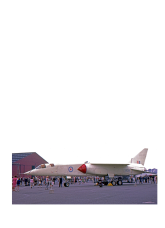
\includegraphics[width=4in]{../figures/TSR_2.jpg}
			\caption{The only BAC TSR-2 prototype to fly, picture taken in 1966 at what is now BAE Warton Lancashire.\protect\footnotemark[1]}
		\end{figure}
		\footnotetext[1]{RuthAS, CC BY 3.0 $<$https://creativecommons.org/licenses/by/3.0$>$, via Wikimedia Commons}	
	\end{vibration_case_study}

	\begin{review}
		Newton's three laws of motion:
		\begin{enumerate}
			\item In an inertial frame of reference, an object either remains at rest or continues to move at a constant velocity unless acted upon by a force.
			\item In an inertial reference frame, the vector sum of the forces $F$ on an object is equal to the mass m of that object multiplied by the acceleration of the object: $F = ma$. (It is assumed here that the mass m is constant)
			\item When one body exerts a force on a second body, the second body simultaneously exerts a force equal in magnitude and opposite in direction on the first body.
		\end{enumerate}
	\end{review}

	\subsection{Single Degree-of-Freedom Systems}
	
        In its simplest form, the phenomenon of vibration is the exchange of energy between potential and kinetic energy. Therefore, a vibrating system must have a component that stores potential energy. This component must also be capable of releasing the energy as kinetic energy. This kinetic energy is stored in the movement of a mass where the measure of this movement is the velocity of the system and the continuous interchange between potential and kinetic energy is the vibration of the system. The simplest vibrating systems can be modeled as a single-degree-of-freedom (1-DOF) system. In a 1-DOF system, one variable can describe the motion of a system. Potential examples of  1-DOF systems include:
		
		\begin{enumerate}
			\item yo-yo
			\item pogo stick
			\item door swinging on axis
			\item throttle (gas pedal)
		\end{enumerate}
				
		\noindent Variables often used for describing 1-DOF systems are $x(t)$,  $y(t)$,  $z(t)$, and  $\theta(t)$.  Examples of 1-DOF systems are presented in figure \ref{fig:Examples_of_1DOF_systems} where the assumption of small displacements is made. Note: we will often drop the ``$(t)$'' for simplicity in this material. 

		\begin{figure}[H]
			\centering
			\includegraphics[]{../figures/Examples_of_1DOF_systems.png}
			\caption{Examples of single degree of freedom (DOF) systems showing: (a) a vertical spring-mass system; (b) a simple pendulum; and (c) a rotational spring-mass system.}
			\label{fig:Examples_of_1DOF_systems}
		\end{figure}

		\subsubsection{Spring-Mass Model}

			\quotebox{\large{All models are wrong, but some are useful}}{George E.P. Box (1919 - 2013)}	
							
            Newtonian physics describes the motion of particles in terms of displacement $x$, velocity $\dot{x}$, and acceleration $\ddot{x}$ vectors. Moreover, Newton's second law of motion says that the change in the velocity of mass in motion is a product of the force acting on the mass. A simple way to express this phenomenon is through a spring-mass model as presented in figure  \ref{fig:spring_mass_model_with_point_mass}. These spring-mass models neglect the mass of the spring and concentrate all the mass of the system into a single point. Note that in this case the force vector and mass-acceleration vectors lie on the same axis and as such are collinear. Therefore, these vectors can be easily treated as scalers simplifying the math used in the modeling of the system.     

			\begin{figure}[H]
				\centering
				\includegraphics[]{../figures/spring_mass_model_with_point_mass.png}
				\caption{A single-degree-of-freedom (1-DOF) spring-mass model showing: (a) annotated schematic of a mass-spring system; and (b) the equivalent free-body diagram represented as a point-mass system.}
				\label{fig:spring_mass_model_with_point_mass}
			\end{figure}	
		
		\subsubsection{Linear Springs}
	
            Springs are mechanical devices that store energy, moreover, an ideal spring is a theoretical representation of this mechanical device that is massless and responds with a linear increase in force for a unit increase in displacement (i.e. $F=kx$). For simplicity, the springs in the spring-mass models considered in this text are always assumed to be ideal linear springs. A graphical representation of the idealized linear spring is presented in figure \ref{fig:linear_spring_deformation} where a unit force $F$ applied to the free end of the spring results in a unit displacement $x$ of the spring.  The resulting mathematical relationship,  $F=kx$, is known as Hooke's Law. Nonlinear springs add considerable complexity to the modeling of spring-mass systems, therefore, these are not considered in this introductory work. 
			
			\begin{figure}[H]
				\centering
				\includegraphics[]{../figures/linear_spring_deformation.png}
				\caption{Force-displacement plot for a linear spring.}
				\label{fig:linear_spring_deformation}
			\end{figure}					


	\subsection{Equivalent Stiffness}
		
		The generalized concept of stiffness can be directly related to mechanical systems and structural components through Hooke's law. 
		\begin{review}
			Hooke's Law states that the force ($F$) needed to extend or compress a spring by some distance $x$ scales linearly with respect to that distance. This law can be extended to tensional stress of a uniform and elastic bar where the length, area, and Young's modulus of the bar are represented by $l$, $A$, and $E$, respectively. Knowing the tensile stress in the bar:
			\begin{equation}
			\sigma = \frac{F}{A}
			\end{equation} 			
			and the definition of strain:
			\begin{equation}
			\varepsilon = \frac{\Delta l}{l}
			\end{equation} 			
			Hooke's law can be expanded to represent a uniform and elastic bar:
			\begin{equation}
			\sigma = E \varepsilon
			\end{equation} 			
			It follows that the change in length $\Delta l$ can be expressed as:		
			\begin{equation}
			\Delta l = \varepsilon l = \frac{F l}{A E}
			\end{equation} 
			\textbf{Note:} Hooke's law is often expressed using the convention that $F$ is the restoring force exerted by the spring on the applied force at the free end. Defining the stiffness and displacement as $k = \frac{AE}{l}$ and $\Delta l = x$, respectively. The equation for Hooke's Law becomes:
			\begin{equation}
			F = -kx
			\end{equation} 			
			since the direction of the restoring force is opposite the spring displacement.
		\end{review}
	
		\subsubsection{Equivalent Stiffness of Structural Systems}	
		
            For a rod with a uniform cross-section, a direct representation of the system can be developed as expressed in figure \ref{fig:spring_and_bar_mass_vertical} where the vibration along the axis of the rod is to be considered. The stiffness of the rod, $k$, is a measure of the resistance offered by an elastic body to deformation. 

			
			\begin{figure}[H]
				\centering
				\includegraphics[]{../figures/spring_and_bar_mass_vertical.png}
				\caption{Equivalency between a vertical bar with a mass attached to the bottom and a spring-mass model of the system.}
				\label{fig:spring_and_bar_mass_vertical}
			\end{figure}
			
			For this 1-DOF system, the equation of a spring can be rearranged such that the stiffness can be defined as:
			\begin{equation}
				k=\frac{F}{x}
			\end{equation}
			The stiffness of the spring can be more closely related to material properties of the bar $A$, $E$, and $l$ considering that Hooke's Law for the uniform tension on a bar can be expressed as:
			\begin{equation}
				\sigma = E \varepsilon
			\end{equation}			
			This expression can be expanded into the form:
			\begin{equation}
				\frac{F}{A} = E \Big( \frac{x}{l} \Big)
			\end{equation}					
			rearranging the terms and recalling the expression $k = \frac{F}{x}$ leads to:			
			\begin{equation}
				 k = \frac{EA}{l}
			\end{equation}				
		
			In a similar fashion, we can also solve the equivalent system for a mass at the end of a cantilever beam.
			\begin{figure}[H]
				\centering
				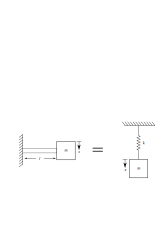
\includegraphics[]{../figures/spring_and_bar_mass_cantilever_beam.png}
			\end{figure}			
			From engineering mechanics, we can compute the deflection at the point of a beam $\delta$ with a point load $P$. This expression is typically expressed as:
			\begin{equation}
				\delta = \frac{Pl^3}{3EI}
			\end{equation}					
			If we transform this equation into our variable system by exchanging $P$ for $F$ and $\delta$ for $x$. Thereafter, the point load is replaced with the equivalent force $F$ generated by the mass and the pull of gravity($mg$). As before, knowing that the stiffness of the system can be expressed as $k=F/x$ we can show that:
			\begin{equation}
				k = \frac{3EI}{l^3}
			\end{equation}	


			\begin{example}
    			
    			Considering the rod diagrammed below; calculate an equivalent spring constant for the rod using the length of the rod $l$, its area $A$, and Young's modulus $E$ for a compressive force $F$ that compresses the rod a distance $x$. Additionally, is a linear spring a useful model for a rod under compression? What if the rod is under tension?
        
		 		\begin{figure}[H]
		 			\centering
		 			\includegraphics[]{../figures/compressed_cantilever_rod.png}
		 			\caption{Compressed cantilever rod. }
		 		\end{figure}	   
       
			    \noindent \textbf{Solution:}

				 The rod shortens by a distance $x$ under the axial force $F$, this can be related to the equation of a linear spring $F=kx$ by recalling from solid mechanics that the elongation (or shortening) of a rod is expressed as 
			
			    \begin{eqnarray}
			    x=\frac{x}{l}l=\varepsilon l = \frac{\sigma}{E}l = \frac{Fl}{AE}
			    \end{eqnarray}    
			    
			    where  $\varepsilon = \frac{x}{l}$ is the strain value and $\sigma = F/A$ is the stress induced in the rod. Combining this expression with the equation of a linear spring yields:
			    
			    \begin{eqnarray}
			    k = \frac{F}{x}= \frac{AE}{l}
			    \end{eqnarray}     
			   
			    As per the usefulness of the linear spring to represent an axial rod under compression or tension, this would be application-specific but could generally be considered an excellent first-order approximation.  
			
			\end{example}

		\subsubsection{Springs in Series and Parallel}
			
			In many cases, it becomes necessary to model a mechanical system as a set of springs (e.g., a composite material, a table with multiple legs).  For these systems, or for systems with more than one spring acting on a body, equivalent stiffness can be calculated as:
			\begin{figure}[H]
				\centering
				\includegraphics[]{../figures/equivalent_stiffness.png}
				\caption{Equations for calculating the equivalent stiffness of two springs ($k_1$ and $k_2$); (a) in series; and (b) in parallel.}
			\end{figure}	
			These are derived considering the displacement $\delta$ of the systems. For two springs in series:
			\begin{figure}[H]
				\centering
				\includegraphics[]{../figures/equivalent_stiffness_series.png}
				\caption{Two springs $k_1$ and $k_2$ combined in series.}
			\end{figure}			
			\noindent where the total displacement is 
			\begin{equation}
				\delta_{ac} = \delta_{ab} + \delta_{bc}
			\end{equation}
			Using the equation for stiffness $k=F/\delta$, this converts to:
			\begin{equation}
				\frac{F}{k_{ac}} = \frac{F}{k_{1}} + \frac{F}{k_{2}}
			\end{equation}
			As $F$ is the same throughout the system, we can cancel out $F$. Solving for the equivalent stiffness yields:
			\begin{equation}
				k_{ac} = \frac{1}{\frac{1}{k_1}+\frac{1}{k_2}}
			\end{equation}
			Similarly for a system of springs in parallel:
			\begin{figure}[H]
				\centering
				\includegraphics[]{../figures/equivalent_stiffness_parallel.png}
				\caption{Two springs $k_1$ and $k_2$ combined in parallel.}				
			\end{figure}			
			\noindent The displacement in both springs is the same, so the total displacement is 
			\begin{equation}
				\delta_{ab} = \delta_{\text{1}} =  \delta_{\text{2}} = \delta
			\end{equation}
			The forces in the direction of spring elongation sum to zero, therefore:
			\begin{equation}
				F_{ab} = F_{\text{1}} +  F_{\text{2}}
			\end{equation}			
			Substituting the displacement and stiffness into the force equation yields:
			\begin{equation}
				\delta k_{ab} = 	\delta k_{1} +  \delta k_{2}
			\end{equation}				
			this simplifies to:
			\begin{equation}
				k_{ab} = k_1+k_2
			\end{equation}
			


			\begin{example}

				Calculate the equivalent stiffness of the following system:
				\begin{figure}[H]
					\centering
					\includegraphics[]{../figures/equivalent_mass_and_spring_system_1.png}
				\end{figure}	
				The springs are combined as shown, using the equations defined before.  Now, considering that the displacement ($\delta$) of the top spring, and the bottom spring are the same we can state the total stiffness $k$, which is the summation of the two. Therefore,    
				\begin{figure}[H]
					\centering
					\includegraphics[]{../figures/equivalent_mass_and_spring_system_2.png}
				\end{figure}	
%				until a final $k$ value can be obtained:
%				\begin{equation}
%					k=k_1+k_2+k_5+\frac{1}{\frac{1}{k_3}+\frac{1}{k_4}}
%				\end{equation}		
				\noindent where the final addition, $(k_1+k_2) + (k_5+\frac{1}{\frac{1}{k_3}+\frac{1}{k_4}})$ is applied at two springs in parallel as each spring is connected between the mass and the fixity. Rearranging this new expression to get a common denominator:
				\begin{equation}
					k= \frac{(k_1+k_2+k_5)(k_3+k_4)+k_3k_4}{k_3+k_4}  
				\end{equation}				
%				For an arbitrary mass, $m$, the undamped frequency $\omega_n$ can be calculated as:
%				\begin{equation}
%					\omega_n = \sqrt{\frac{k}{m}} = \sqrt{\frac{(k_1+k_2+k_5)(k_3+k_4)+k_3k_4}{m(k_3+k_4)} }
%				\end{equation}				
			\end{example}	

					
	\subsection{Equation of Motion for an Oscillating System}			
			
        An Equation of Motion (EOM) is an equation that provides a basis for modeling a vibrating system about its equilibrium point and relates the transfer of the potential energy from the spring to the kinetic energy mass. In developing the EOM we assume that any surfaces are frictionless and as such, no energy is extracted from the vibrating system. Referencing the 1-DOF system in figure \ref{fig:EOM_1-DOF-mass_horizontal}(a), and assuming the mass only moves in the $x$ direction, the only force acting on the mass in the $x$ direction is the force that results from the elongation of the spring as annotated in figure \ref{fig:EOM_1-DOF-mass_horizontal}(b). Therefore, the sum of forces along the $x$ axis must equal the mass ($m$) times the acceleration of the mass ($a\dot{x}$). 

		\begin{figure}[H]
			\centering
			\includegraphics[]{../figures/EOM_1-DOF-mass_horizontal.png}
			\caption{A spring-mass model of a 1-DOF system showing: (a) a schematic of the system; (b) a free-body diagram of the system at its initial position.}
			\label{fig:EOM_1-DOF-mass_horizontal}
		\end{figure}			
		
		Considering that positive displacements are to the right, the standard form of the equation of motion for an undamped system without any excitation is expressed as:  
		\begin{equation}
			s_1 \ddot{x} + s_2 x = 0
		\end{equation}			
		where $s_1$ and $s_2$ are constants to be determined for the specific system. A systematic approach to obtaining the free-body diagram (FBD) of a system under vibration can be expressed in three steps:
		\begin{enumerate}
			\item Draw a free-body diagram (FBD) at the system's equilibrium and displaced position (without a displacing force).
			\item Apply Newton's second law to both FBDs ( equilibrium and displaced).
			\item Combine the equations to write the EOM in standard form with the forcing component on the right-hand side. For free vibration, the forcing component is 0. 
		\end{enumerate}
			
		Solving these three steps for 1-DOF system presented in figure \ref{fig:EOM_1-DOF-mass_horizontal} results in the EOM:
		\begin{equation}
			m \ddot{x} + k x = 0
		\end{equation}

		\begin{review}
			A second-order linear homogeneous differential equation has the form:
			
			\begin{equation}
			 a \ddot{x} + b \dot{x} + cx = 0
			\end{equation}
		
			\noindent The EOM for a 1-DOF system under a free vibration is a second-order differential equation due to acceleration ($\ddot{x}$) being the second derivative of displacement ($x$) and homogeneous as the forcing function (right-hand side of the equations) is zero. In EOM's current form, $a=m$, $b=0$,  and $c=k$. In future work, $b$ will account for damping in the vibrating system.     
		\end{review}

					
		\begin{example}			
			
			Considering the system:
			\begin{figure}[H]
				\centering
				\includegraphics[]{../figures/1-DOF-spring_mass_horizontal.png}
			\end{figure}		
			
			\textbf{Step-1}
			Define the direction of displacement, and draw the FBD for the equilibrium and displaced state.  
			\begin{figure}[H]
				\centering
				\includegraphics[width=0.45\textwidth]{../figures/1-DOF-mass_horizontal_FBD.png}\\
				equilibrium state \hspace{3cm} displaced state
			\end{figure}		
			\noindent The equation for the equilibrium state is:
			\begin{equation}
			\rightplus \sum F_x = 0
			\end{equation}
			and in the displaced state:
			\begin{equation}
			\rightplus \sum F_x = -kx
			\end{equation}		
			This equation does not equal zero as the FBD does not account for the restoring force. 
	
			\noindent	\textbf{Step-2} Apply Newton's second law (we want to store energy in the kinetic state) of motion to the sum of forces for the displaced position we get: 		 		
			\begin{equation}
			ma = m\ddot{x} = \rightplus \sum F_x = -kx
			\end{equation}			
			\begin{equation}
			m\ddot{x} = -kx
			\end{equation}				
			\textbf{Step-3} Rearrange in the Equation to construct an EOM: 			
			\begin{equation}
			m\ddot{x} + kx = 0
			\end{equation}		
		\end{example}			

		\begin{example}	
			Some systems will have an initial displacement, as the system will oscillate around this position we need to define the EOM about this position. Considering the system:
			\begin{figure}[H]
				\centering
				\includegraphics[]{../figures/1-DOF-spring_mass_vertical.png}
			\end{figure}		
			\noindent \textbf{Step-1}
			Define the direction of displacement, and draw the FBD for the equilibrium and displaced state.  
			\begin{figure}[H]
				\centering
				\includegraphics[]{../figures/1-DOF-spring_mass_vertical_FBD.png}\\
				equilibrium state \hspace{3cm} displaced state
			\end{figure}		
			\noindent The equation for the equilibrium state is:
			\begin{equation}
				\downplus \sum F_x = mg - k\delta = 0
			\end{equation}
			and in the displaced state:
			\begin{equation}
				\downplus \sum F_x =mg -k(\delta + x)
			\end{equation}	
			This equation does not equal zero as the FBD does not account for the restoring force.	
			
			\noindent \textbf{Step-2} Apply Newton's second law (we want to store energy in the kinetic state) of motion to the sum of forces for the displaced position we get: 		
			\begin{equation}
				m\ddot{x} = \downplus \sum F_x =mg -k\delta -kx
			\end{equation}
			We can than use the information from the equilibrium state to cancel out some terms, this becomes:
			\begin{equation}
				m\ddot{x} = -kx
			\end{equation}				
			\textbf{Step-3} Rearrange in the Equation to construct an EOM: 					
			\begin{equation}
				m\ddot{x} + kx = 0
			\end{equation}			
		\end{example}		


		\begin{vibration_case_study}
			Why study vibrations? One day, it could save your job! For a project to be successful they need to be completed on time and within budget. Consider the Ling-Temco-Vought (LTV) XC-142  which was a tilt-wing experimental aircraft developed in the '60s for the US military and later turned over to NASA. During testing, the cross-linked driveshaft produced excessive vibration and noise which resulted in a high pilot workload. In general, the aircraft's cross-linked driveshaft was the main technical issue that caused the military to lose interest in the project. 
			
			\begin{figure}[H]
				\centering
				\includegraphics[width=4in]{../figures/Ling_Temco_Vought_XC_142A.jpg}
				\caption{A Ling-Temco-Vought XC-142A tested at the NASA Langley Research Center in 1969. \protect\footnotemark[1]}
			\end{figure}
			\footnotetext[1]{NASA,  Photograph published in Winds of Change, 75th Anniversary NASA publication, by James Schultz, Public domain, via Wikimedia Commons}	
		\end{vibration_case_study}


	
\end{document}



% Chapter 2 Free Vibrations
\include{Chapter_2_free_vibration/Chapter_2_free_vibration}

% Chapter 3 Forced Vibrations
\include{Chapter_3_forced_vibration/Chapter_3_forced_vibration}

% Chapter 4 Transfer Function
\include{Chapter_4_transfer_function/Chapter_4_transfer_function}

% Chapter 5 Multiple DOF Systems
\documentclass[12pt,letter]{article}
\usepackage{mathptmx} % added for time new roman font
\usepackage[left=1in,right=1in,top=1in,bottom=1in]{geometry}
\usepackage[latin1]{inputenc}
\usepackage{amsmath}

% defines all example enviorment
\usepackage[framemethod=tikz]{mdframed} % added for the box around examples
\newtheorem{ex}{Example}
\numberwithin{ex}{section} % allows for the use of example numbers that lign up with the section numbers
\newenvironment{example}{\begin{mdframed}[middlelinewidth=0.5mm]\begin{ex}\normalfont}{\end{ex}\end{mdframed}}

% defines all review enviorment
\usepackage[framemethod=tikz]{mdframed} % added for the box around examples
\newtheorem{re}{Review}
\numberwithin{re}{section} % allows for the use of example numbers that lign up with the section numbers
\newenvironment{review}{\begin{mdframed}[middlelinewidth=2mm,roundcorner=20pt]\begin{re}\normalfont}{\end{re}\end{mdframed}}

% defines all vibration case studies
\newtheorem{vcs}{Vibration Case Studies}
\numberwithin{vcs}{section} % allows for the use of numbers that lign up with the section numbers
\newenvironment{vibration_case_studies}{\begin{mdframed}[linecolor=orange,middlelinewidth=2mm,roundcorner=20pt]\begin{vcs}\normalfont}{\end{vcs}\end{mdframed}}

% defines the quotation enviorment 
\usepackage{xcolor}
\newcommand{\quotebox}[2]{\begin{center}\fcolorbox{white}{blue!15!gray!15}{\begin{minipage}{0.9\linewidth}\vspace{10pt}\center\begin{minipage}{0.8\linewidth}{\space\Huge``}{#1}{\Huge''}{\break\null\hfill} {\small #2}  \end{minipage}\medbreak\end{minipage}}\end{center}}

% defines the definition enviorment 
\newcommand{\definitionbox}[2]{\begin{center}\fcolorbox{white}{blue!15!gray!15}{\begin{minipage}{0.9\linewidth}\vspace{10pt}\center\begin{minipage}{0.8\linewidth} {{\textbf{Definition} - }{#1}: {#2}}\end{minipage}\medbreak\end{minipage}}\end{center}}

\usepackage{amsfonts}
\usepackage{amssymb}
\usepackage{graphicx}
\usepackage{float}
\usepackage{booktabs}
%\usepackage{parskip} % remove all the paragraph indents
\usepackage[textsize=tiny]{todonotes}


\usepackage{setspace}
\usepackage[colorlinks=true]{hyperref}
\usepackage{textcomp} 
\usepackage{multicol} 

% added for MATLAB code
\usepackage[framed]{matlab-prettifier}
\let\ph\mlplaceholder % shorter macro
\lstMakeShortInline"

\lstset{
	style              = Matlab-editor,
	basicstyle         = \mlttfamily,
	escapechar         = ",
	mlshowsectionrules = true,
}



\usepackage{color} % color added for editing
\newcommand{\bl}[1]{\textcolor[rgb]{0.00,0.00,1.00}{#1}}
\newcommand{\gr}[1]{\textcolor[rgb]{0.00,0.50,0.00}{#1}}
\newcommand{\rd}[1]{\textcolor[rgb]{0.75,0.00,0.00}{#1}}
\newcommand{\tl}[1]{\textcolor[rgb]{0,0.6,0.60}{#1}}



%%%%%%%		define the symbols for positive directions		%%%%%%
\makeatletter													%%	
%%					
\newcommand*\curveplus{% positive counterclockwise				%%
	\mathbin{\rotatebox[origin=c]{90}{$\m@th\curvearrowleft$}+}}	%%
%%
\newcommand*\rightplus{% positive right							%%
	\mathpalette\@rightplus\relax}								%%
\newcommand*\@rightplus[1]{%									%%
	\mathbin{\vcenter{\hbox{$\m@th\overset{#1+}{\to}$}}}}			%%
%%	
\newcommand*\upplus{% positive up								%%
	\mathbin{+\mathord\uparrow}}									%%
%%			
\newcommand*\downplus{% positive down							%%		
	\mathbin{+\mathord\downarrow}}								%%
%%		
\newcommand*\downrightplus{% positive down and right			%%	
	\mathbin{+ \rotatebox[origin=c]{-30}{$\m@th\rightarrow$}}}	%%
\makeatother 													%%	
%%%%%%%%%%%%%%%%%%%%%%%%%%%%%%%%%%%%%%%%%%%%%%%%%%%%%%%%%%%%%%%%%%


\usepackage{mathtools}          %loads amsmath as well added for the piece wise function
\DeclarePairedDelimiter\Floor\lfloor\rfloor
\DeclarePairedDelimiter\Ceil\lceil\rceil


\newcounter{NumberInTable}
\newcommand{\LTNUM}{\stepcounter{NumberInTable}{(\theNumberInTable)}}

\newcommand{\Laplace}[1]{\ensuremath{\mathcal{L}{\left[#1\right]}}}
\newcommand{\InvLap}[1]{\ensuremath{\mathcal{L}^{-1}{\left[#1\right]}}}
\renewcommand{\textuparrow}{$\uparrow$}

% Sets the footnotes to be letters, not numbers. This is needed or it's a mix of both. 
\renewcommand*\thefootnote{\alph{footnote}}


\begin{document}
	
	% set the section number, along with figure and equation numbers
	\setcounter{section}{4}	
	\setcounter{figure}{0}   
	\renewcommand\thefigure{\thesection.\arabic{figure}}
	\setcounter{equation}{0}   
	\renewcommand\theequation{\thesection.\arabic{equation}}
	
	\section{Multiple degree-of-freedom systems}



Until now we have only considered and modeled systems that can require one coordinate system to describe their motion. In this chapter, we will develop the mathematical tools required to model multiple degree-of-freedom systems that require multiple independent coordinates to describe their motion. As before, the equations that describe the motion of rigid bodies in space are developed from Newton's second law of motion. However, unlike before, there exists an independent equation for each body in motion. These equations are therefore coupled by the system and are often expressed in matrix notation such that the mass, damping, and stiffness matrices are easily defined. 




\begin{review}
\textbf{Linear Algebra}

Linear algebra allows for the efficient solving of these coupled equations. In this text, matrices are expressed as bold capital letters ($\textbf{X}$), vectors are denoted with an arrow ($\vec{x}$), and scalars and italic letters ($x$). However, given the range of notation needed, it is not always possible to strictly follow this formulation.

The dot product allows us to multiply matrices and is defined as:
\begin{eqnarray}
  \begin{bmatrix} a & b \\ c & d \end{bmatrix}\begin{bmatrix} e \\  f \end{bmatrix} = \begin{bmatrix} ae+bf \\ ce + df \end{bmatrix}
\end{eqnarray}
Another arrangement of the same principle, in a format more related to vibrations, is:
\begin{eqnarray}
  \begin{bmatrix} a_1+a_2 & b \\ c & d \end{bmatrix}\begin{bmatrix} e \\  f \end{bmatrix} = \begin{bmatrix} (a_1+a_2)e+bf \\ ce + df \end{bmatrix}
\end{eqnarray}

The transpose of a matrix is an operator which flips a matrix over its diagonal. For a matrix $\textbf{A}$, the transpose $\textbf{A}^\text{T}$ can be written as:
\begin{eqnarray}
   \textbf{A} = \begin{bmatrix} a & b \\ c & d \\ e & f\end{bmatrix} \rightarrow \textbf{A}^\text{T} = \begin{bmatrix} a & c & e \\  b & d & f \end{bmatrix}
\end{eqnarray}

A matrix is symmetric if $\textbf{A} =\textbf{A}^\text{T}$. Therefore, the symmetric matrix must be square and can be written as:
\begin{eqnarray}
   \textbf{A} = \begin{bmatrix} a & b &c \\ d & e & f\\ g & h & i \end{bmatrix} = \textbf{A}^\text{T} = \begin{bmatrix} a & d & g \\ b & e & h \\ c & f & i \end{bmatrix}\text{, where } b=d \text{, }c=g\text{, }f=h
\end{eqnarray}

The determent of a matrix is a scalar value that is a function of the entries of a square matrix. The determent characterizes the matrix and its linear map. The determent is often writted as det($\textbf{A}$), det $\textbf{A}$, or $|\textbf{A}|$. For a 2 $\times$ 2 matrix this is defined as:
\begin{eqnarray}
\det (\textbf{A}) = ad-bc  \text{, when } \textbf{A} = \begin{bmatrix} a & b \\ c & d \end{bmatrix}
\end{eqnarray}

The inverse of a square matrix is such that $\textbf{A}\textbf{A}^{-1} = \textbf{A}^{-1}\textbf{A}=\textbf{I}$ where $\textbf{I}$ is the identity matrix:
\begin{eqnarray}
\textbf{I} = \begin{bmatrix} 1 & 0 \\ 0 & 1 \end{bmatrix} 
\end{eqnarray}
and the inverse of a 2 $\times$ 2 matrix is defined as:
\begin{eqnarray}
\textbf{A}^{-1} = \frac{1}{\det (A)} \begin{bmatrix} d & -b \\ -c & a \end{bmatrix} \text{, when } \textbf{A} = \begin{bmatrix} a & b \\ c & d \end{bmatrix}
\end{eqnarray}

A matrix that does not have an inverse is called a singular matrix.


\end{review}

\subsection{General Discussion on Mode Shapes}

Studying and characterizing the natural frequencies of a system allows for the detailed investigation of the system response. Modern vibration analysis relies heavily on the concepts of mode shapes for various engineering tasks. Particle applications of the study of mode shapes (often called experimental modal analysis) include
\begin{itemize}
	\item Correlation Finite Element Analysis with structures
	\item Structural Dynamic Modification
	\item Reduction of Finite Element Analysis models
	\item Forced Response Prediction			
	\item Active Vibration Control	
\end{itemize}

\begin{vibration_case_studies}
	In automotive engineering, the requirements for safe and comfortable vehicles necessitate the need for a thorough understanding of the vehicle's dynamic properties and how and any design changes affect its dynamics. Experimental modal analysis is an important troubleshooting and model updating tool in the study of vehicle noise and vibration harshness (NVH). Oftentimes, experimental modal analysis is performed on a ``body in white'' or a sub-frame structure to develop a better understanding of the dynamics of the structure. Overall, experimental modal analysis is an important tool used in improving a vehicle's NVH performance.
	\begin{figure}[H]
		\centering
		\includegraphics[width=6in]{../figures/modal_testing}
		\caption{Experimental modal analysis of an automotive (Jaguar) body in white, typically done to reduce vehicle noise and vibration harshness \protect\footnotemark[1].}
	\end{figure}
	\footnotetext[1]{Cjp24, CC BY-SA 3.0 $<$https://creativecommons.org/licenses/by-sa/3.0$>$, via Wikimedia Commons} 	
\end{vibration_case_studies}



 

Mode shapes are not the displacement of a system, rather they describe the configurations into which a structure will naturally displace at a given frequency. For example, consider the 4-DOF system shown in figure~\ref{fig:general_mode_shapes} that represents a pole (i.e. cantilever beam). Assuming that the system experience a linear response and using the mode-superposition method we can see that the displaced shape $\vec{x}$ is a function of all of the mode shapes $u_i$ and their corresponding participation factors $q_i$. Note that the mode shapes associated with the lower frequencies tend to provide the greatest contribution to structural response. As the frequencies that excite the modes increase, the mode shapes contribute less, are predicted less reliably, and are harder to measure. Therefore, the analysis of the system is often truncated after the first few modes and rarely exceeds the 10$^{\text{th}}$ mode. 

Figure~\ref{fig:general_mode_shapes} shows a structure with $N$ degrees of freedom that therefore had $N$ corresponding mode shapes. Each mode shape is independent and normalized such that the maximum displacements are the same. The summation of the mode shapes multiplied by their corresponding participation factors ($q_i$) yields the deflection of the structure. 


\begin{figure}[H]
	\centering
	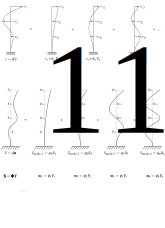
\includegraphics[]{../figures/general_mode_shapes.png}
	\caption{Deflection of a vertical cantilever, $\vec{x}$, is a function of the considered mode shapes $u_i$ and their corresponding participation factors $q_i$.}
	\label{fig:general_mode_shapes}
\end{figure}





\subsection{Modeling Undamped Two Degree of Freedom Systems}
\label{sec:two_degree_of_freedom}

Consider the undamped 2-DOF systems presented in figure \ref{fig:2-DOF-spring_mass_examples}. This system with a single mass capable of moving in two directions. To expand, figure \ref{fig:2-DOF-spring_mass_examples}(a) reports a mass that can move horizontally or vertically in space. However, this mass does not rotate during its movements. Moreover, figure \ref{fig:2-DOF-spring_mass_examples}(b) presents a system that rotates about the spring and displaces vertically. These are examples of 2 DOF systems because each system has two independent coordinate systems that express the movement of the mass. 

\begin{figure}[H]
	\centering
	\includegraphics[]{../figures/2-DOF-spring_mass_examples.png}
	\caption{Examples of single mass 2-DOF systems that: (a) displace in the vertical and horizontal directions; and (b) rotates about the spring and displaces in the vertical direction. }
	\label{fig:2-DOF-spring_mass_examples}
\end{figure}

Another example of a 2-DOF system with two masses, each with their own independent coordinate system, is presented in figure \ref{fig:2-DOF-spring_mass_horizontal}. The two coordinates that describe the system's movements are $x_1$ and $x_2$.

\begin{figure}[H]
	\centering
	\includegraphics[]{../figures/2-DOF-spring_mass_horizontal.png}
	\caption{2-DOF system with two masses and two independent confidante systems $x_1$ and $x_2$.}
	\label{fig:2-DOF-spring_mass_horizontal}
\end{figure}

\subsubsection{Solution for the Two-Degree-of-Freedom System}
Before we derive a model for undamped 2-DOF systems, let us first consider the solution to the system shown in figure \ref{fig:2-DOF-spring_mass_horizontal}. The solution consists of two equations, one for each mass. This solution will be derived in section \ref{sec:2-DOF_derive_solution} and is expressed by the coupled equations:
\begin{equation}
	x_1(t) = A_1 \sin (\omega_1 t + \phi_1 )u_{11}+ A_2 \sin (\omega_2 t + \phi_2 )u_{12} \hspace{3.35cm} 
\end{equation}
\begin{equation}
	x_2(t) = A_1 \sin (\omega_1 t + \phi_1 )u_{21}+ A_2 \sin (\omega_2 t + \phi_2 )u_{22} , \hspace{1cm} \omega_1 \text{ or } \omega_2 \neq 0 \nonumber
\end{equation}
These two equations ban be written as a single equation in matrix form as:
\begin{equation}
	\vec{x}(t) = A_1 \sin (\omega_1 t + \phi_1 )\vec{u}_1 + A_2 \sin (\omega_2 t + \phi_2 )\vec{u}_2 , \hspace{1cm} \omega_1 \text{ or } \omega_2 \neq 0
	\label{eq:2-DOF_solution}
\end{equation}
Where the bold text denotes vectors. Therefore, the vectors $\vec{u}_1$ and $\vec{u}_2$ are the mathematical expressions that ``couple'' or tie the equations together. Expanding these vectors shows: 
\begin{eqnarray}
 \vec{x}(t)=  \begin{bmatrix} x_1(t) \\  x_2(t) \end{bmatrix}, \hspace{2ex} \vec{u}_1=  \begin{bmatrix} u_{11} \\  u_{21} \end{bmatrix}, \hspace{2ex} \vec{u}_2=  \begin{bmatrix} u_{12} \\  u_{22} \end{bmatrix}\text{, }
\end{eqnarray}
The four key components of the solution expressed in equation \ref{eq:2-DOF_solution} are:
\begin{enumerate}
\item $\omega_1$ and $\omega_2$ are the natural frequencies of the system. They are not the frequencies of the masses. The solution states that each of the masses oscillates at the two frequencies $\omega_1$ and $\omega_2$. Moreover, consider the special case where the initial conditions are selected to force $A_2 = 0$, in this case, each mas would only oscillate at only one frequency, $\omega_1$.
\item $A_1$ and $A_2$ are the constants of integration and determine the amplitude of the system.
\item $\phi_1$ and $\phi_2$ represents the phase shift of the system
\item $\vec{u}_1$ and $\vec{u}_2$ are the first and second mode shapes of the system and couple the system together.
\end{enumerate}

\subsubsection{Deriving the Solution for the Two-Degree-of-Freedom System}
\label{sec:2-DOF_derive_solution}
To derive this solution for the system under consideration a FBD for figure \ref{fig:2-DOF-spring_mass_horizontal} can be constructed for the forces acting on each mass. First we have to make the assumption that $x_1 < x_2$, this allows us to say that $m_2$ pulls on $m_1$ and results in:
\begin{figure}[H]
	\centering
	\includegraphics[]{../figures/2-DOF-spring_mass_horizontal_FBD.png}
	\caption{Free body diagram for the 2-DOF system presented in figure \ref{fig:2-DOF-spring_mass_horizontal}.}
	\label{fig:2-DOF-spring_mass_horizontal_FBD}
\end{figure}
\noindent Applying Newton's second law and summing the forces on each mass in the horizontal direction yields:
\begin{eqnarray}
m_1\ddot{x}_1 &= & -k_1x_1 + k_2(x_2-x_1) \\
m_2\ddot{x}_2&= & -k_2(x_2-x_1)  \nonumber
\end{eqnarray}
These equations can be rearranged in terms of  $x_1$ and $x_2$ as:
\begin{eqnarray}
m_1\ddot{x}_1 +(k_1+k_2)x_1 -k_2x_2 =0 \\
m_2\ddot{x}_2 - k_2x_1 + k_2x_2 = 0 \nonumber
\end{eqnarray}
where these are two coupled second-order differential equations that each require two initial conditions to solve. These initial conditions can be obtained form the displacement and velocity terms as:
\begin{eqnarray}
x_1(0) = x_{10} \\
\dot{x}_1(0) = \dot{x}_{10} = v_{10} \nonumber \\ 
x_2(0) = x_{20} \nonumber \\ 
\dot{x}_2(0) = \dot{x}_{20} = v_{20} \nonumber
\end{eqnarray}
As before, these initial conditions will be the constants of integration used to solve the two second-order differential equations. This solution will provide the free response of each mass in the system. There is a multitude of ways to solve these two coupled second-order differential equations, however, here we will just consider a matrix notation solution. This matrix notation solution is used as this formulation is readably solved using computers and is expandable to more than 2 DOF.

To initiate the solution, let us first develop the matrix formulation of the two coupled ODEs:
\begin{eqnarray}
  \begin{bmatrix} m_1 & 0  \\  0 & m_2 \end{bmatrix}\begin{bmatrix} \ddot{x_1} \\  \ddot{x_2} \end{bmatrix} + \begin{bmatrix} k_1+k_2 & -k_2  \\  -k_2 & k_2 \end{bmatrix}\begin{bmatrix} x_1 \\  x_2 \end{bmatrix} = \begin{bmatrix} 0 \\  0 \end{bmatrix}
\end{eqnarray}
This equation can also be expressed as the vector equation:
\begin{equation}
M\ddot{\vec{x}} + K\vec{x} =0
\end{equation}
and is known as the EOM in vector form. In this formulation the mass matrix ($M$) is defined as:
\begin{eqnarray}
 M=  \begin{bmatrix} m_1 & 0  \\  0 & m_2 \end{bmatrix}  
\end{eqnarray}
while the stiffness matrix ($K$) is:
\begin{eqnarray}
 K=  \begin{bmatrix} k_1+k_2 & -k_2  \\  -k_2 & k_2 \end{bmatrix}
\end{eqnarray}
along with the displacement, velocity, and acceleration matrices:
\begin{eqnarray}
 \vec{x}=  \begin{bmatrix} x_1 \\  x_2 \end{bmatrix} , \hspace{2ex} \dot{\vec{x}}=  \begin{bmatrix} \dot{x}_1 \\  \dot{x}_2 \end{bmatrix}, \hspace{2ex} \ddot{\vec{x}}=  \begin{bmatrix} \ddot{x}_1 \\  \ddot{x}_2 \end{bmatrix}
\end{eqnarray}
Beyond these equations, we can write the initial conditions as:
\begin{eqnarray}
\vec{x}_0=  \begin{bmatrix} x_1(0) \\  x_2(0) \end{bmatrix},  \hspace{1cm} \dot{\vec{x}}_0=  \begin{bmatrix} \dot{x}_1(0) \\  \dot{x}_2(0) \end{bmatrix}
\end{eqnarray}
This simple connection between vibration analysis and matrix analysis allows computers to be used to solve large and complicated vibration problems quickly.

Recall that the 1-DOF version of the equation of motion was solved by calculating the values of the constants in an assumed harmonic solution. The same approach is applied here in order to solve for the displacement of the two-DOF system. This time, the solution is assumed in the form:

\begin{equation}
	\vec{x}(t) = \vec{u}e^{j\omega t}
\end{equation}
where $\vec{u}$ is a vector of constants to be demerited and can be written as:
\begin{eqnarray}
\vec{u}=  \begin{bmatrix} u_1 \\  u_2 \end{bmatrix}
\end{eqnarray}
From before, $\omega$ is also a constant to be determined. Again, $j=\sqrt{-1}$. In the same manner as before, $e^{j\omega t}$ represents harmonic motion as $e^{j\omega t} = \cos(\omega t) + j \sin(\omega t)$. Taking the derivatives of $\vec{x}(t) = \vec{u}e^{j\omega t}$ yields:
\begin{equation}
	\dot{\vec{x}}(t) = j\omega\vec{u}e^{j\omega t}
\end{equation}
\begin{equation}
	\ddot{\vec{x}}(t) = -\omega^2\vec{u}e^{j\omega t}
\end{equation}
Substituting this into the EOM in vector form ($M\ddot{\vec{x}} + K\vec{x} =0$) yields:
\begin{equation}
-\omega^2 M  \vec{u}e^{j\omega t} + K\vec{u}e^{j\omega t} =0
\end{equation}
or 
\begin{equation}
(-\omega^2 M  + K)\vec{u}e^{j\omega t} =0
\end{equation}
As $e^{j\omega t} \neq 0$ for any value of $t$ and not allowing $\vec{u}$ to be zero it can be demerited that $(-\omega^2 M  + K)$ must satisfy the vector equation. Therefore,
\begin{equation}
(-\omega^2 M  + K)\vec{u} =0, \hspace{1cm} \vec{u}\neq0
\end{equation}
This forms a homogeneous set of algebraic equations. To be useful, these equations have a nonzero solution for the system must exist. For this to be true, the inverse of the coefficient matrix $(-\omega^2 M  + K)$ must not exist. To expand, assume that the inverse of $(-\omega^2 M  + K)$ does exist, by multiplying both sides of the equation by $(-\omega^2 M  + K)^{-1}$ yields $\vec{u}=0$. This is a trivial solution (it is not useful) as no motion in the system is implied. Therefore, the logical connection can be drawn between the solution of the equation and the inverse of the coefficient matrix $(-\omega^2 M  + K)$.

Applying the singularity condition to the coefficient matrix of equation $(-\omega^2 M  + K)\vec{u} =0, \hspace{1ex} \vec{u}\neq0$ results a nonzero solution of $\vec{u}$. However, for this to exist the following must be true:
\begin{equation}
\det(-\omega^2 M  + K) = 0
\end{equation}
Solving this expression results in one algebraic equation with one unknown ($\omega$). Expanding the above equation to consider the values for the matrices $M$ and $K$ results in:
\begin{eqnarray}
\det\begin{bmatrix} -\omega^2 m_1 + k_1 + k_2 & -k_2  \\  -k_2 & -\omega^2 m_2 + k_2 \end{bmatrix}=0
\end{eqnarray}
Using the definition of the determinant yields that the unknown quantity $\omega^2$ must satisfy:
\begin{equation}
m_1 m_2 \omega^4 - (m_1 k_2 + m_2 k_1 + m_2 k_2)\omega^2 + k_1 k_2 = 0
\label{eq:characteristic_equation}
\end{equation}
This expression is called the characteristic equation for the system and is used to determine the constants $\omega_{1,2}$, in the assumed form of the solution given by the assumed solution $\vec{x}(t) = \vec{u}e^{j\omega t}$, once the values of the physical parameters $m_1$, $m_2$, $k_1$, and $k_2$ are known. Note that $\omega_{1,2}$ are not in the characteristic equation, therefore, solving for $\omega_{1,2}$  will be done by factoring the equation above to obtain two solutions $\omega_1$ and $\omega_2$. The characteristic equation is in the form of the quadratic formula if you set $x=\omega^2$, as:
\begin{equation}
ax^2 + bx +c = 0
\end{equation}

After finding the value of $\omega_{1,2}$ using the characteristic equation, the values in $\vec{u}$ can be found using equation $(-\omega^2 M  + K)\vec{u} =0, \hspace{1ex} \vec{u}\neq0$ for each value of $\omega^2$. That is, for both $\omega_1$ and $\omega_2$ there is a vector  $\vec{u}$ that satisfies the equation. These solutions can be written as:
\begin{equation}
	(-\omega_1^2 M  + K)\vec{u}_1 =0
\end{equation}
and 
\begin{equation}
	(-\omega_2^2 M  + K)\vec{u}_2 =0
\end{equation}
The direction of the vectors $\vec{u}_1$ and $\vec{u}_2$ can be obtained by solving the above expressions, however, the information regarding the magnitude of is not contained in this expression. To verify this, assume that $\vec{u}_1$ satisfies the equation, therefore, the vector $a\vec{u}_1$ also satisfies the equation where $a$ is any nonzero number. Hence the vectors satisfying the above are of arbitrary magnitude.
 
The values obtained for $\vec{u}_1$ and $\vec{u}_2$ can now be combined with the assumed solution:
\begin{equation}
	\vec{x}(t) = \vec{u}e^{j\omega t}
\end{equation}
to form a set of solutions:
\begin{equation}
	\vec{x}(t) = \vec{u}_1e^{-j\omega_1 t}, \hspace{2ex} \vec{u}_1e^{j\omega_1 t}, \hspace{2ex} \vec{u}_2e^{-j\omega_2 t}, \hspace{2ex} \vec{u}_2e^{j\omega_2 t}
\end{equation}
Since the equation to be solved is linear, the solution is the sum of these solutions. This results in:
\begin{equation}
	\vec{x}(t) = (a e^{j\omega_1 t} + b e^{-j\omega_1 t})\vec{u}_1 +(c e^{j\omega_2 t} + d e^{-j\omega_2 t})\vec{u}_2
\end{equation}
where $a$, $b$, $c$, and $d$ are the arbitrary constants of integration to be determined by the initial conditions. Applying Euler's formulas for the sin functions (where $\omega_1 \text{ or } \omega_2 \neq 0$) reorganizes this equation as:
\begin{equation}
	\vec{x}(t) = A_1 \sin (\omega_1 t + \phi_1 )\vec{u}_1 + A_2 \sin (\omega_2 t + \phi_2 )\vec{u}_2 , \hspace{1cm} \omega_1 \text{ or } \omega_2 \neq 0
\end{equation}
Another way to write this equation is in the form:
\begin{equation}
	 \begin{bmatrix} x_1(t) \\  x_2(t) \end{bmatrix} =  \begin{bmatrix} \vec{u}_1 & \vec{u}_2 \end{bmatrix}
	 \begin{bmatrix} A_1 \sin (\omega_1 t + \phi_1 )\\ A_2 \sin (\omega_2 t + \phi_2 )\end{bmatrix}, \hspace{1cm} \omega_1 \text{ or } \omega_2 \neq 0
\end{equation}
Where the values for $A_1$ and $A_2$ can be obtained by setting applying the boundary conditions and taking the derivatives of the equations as done in the 1-DOF problems. 

The final form of the equation provides physical insight into the solution of the system. It states that each mass in the system oscillates at both of the natural frequencies of the system ($\omega_1$ and $\omega_2$). Furthermore, the importance of the initial conditions can be understood. Assume that initial conditions are chosen that result in $A_2=0$, this cancels out the second natural frequency such that each mass oscillates at only one frequency,  $\omega_1$. Moreover, the positions of the masses can be determined by the values of the vector $\vec{u}_1$ at any given time. For this reason,  $\vec{u}_1$ is termed the first mode shape of the system. Likewise, if the opposite initial conditions are chosen such that  $A_1=0$, then both system coordinates (e.g., masses in the systems we have studied) will oscillate at $\omega_2$ and again, the positions can be obtained from the vector $\vec{u}_2$. Where $\vec{u}_2$ is termed the second mode shape. The interactions between mode shapes and natural frequencies are very important and form the basis of several areas in the field of vibrations.

\begin{example}
\label{ex:2-DOF}
Considering the following system:
\begin{figure}[H]
	\centering
	\includegraphics[]{../figures/2-DOF-spring_mass_horizontal.png}
	\caption{2-DOF system with two masses and two independent confidante systems $x_1$ and $x_2$.}
\end{figure}
Calculate response for the system if $m_1$=9 kg, $m_2$=1 kg, $k_1$ = 24 N/m, and $k_2$ = 3 N/m with the initial conditions $x_{10}=1$ mm, $v_{10}=0$ mm/s, $x_{20}=0$ mm, and $v_{20}=0$ mm/s. \\


\noindent \textbf{Solution:} We have already obtained a characteristic equation for this system. This is shown in Equation~\ref{eq:characteristic_equation} and is given as:
\begin{equation}
m_1 m_2 \omega^4 - (m_1 k_2 + m_2 k_1 + m_2 k_2)\omega^2 + k_1 k_2 = 0
\end{equation}
Substituting our values into this obtains:
\begin{equation}
9 \cdot 1 \omega^4 - (9 \cdot 3 + 1 \cdot 24 + 1 \cdot 3)\omega^2 + 24 \cdot 3 = 0
\end{equation}
or
\begin{equation}
\omega^4 - 6\omega^2 + 8 =0
\end{equation}
This can then be factored into:
\begin{equation}
(\omega^2-2)(\omega^2-4)=0
\end{equation}
This results in solutions of $\omega^2_1 = 2$ and $\omega^2_2 = 4$. Leading to:
\begin{equation}
\omega_1 = \pm \sqrt{2} \text{ rad/sec}, \hspace{2ex} \omega_2 = \pm 2 \text{ rad/sec}
\end{equation}
Next, we need to obtain solutions for $\vec{u}_1$ and $\vec{u}_2$. Having solved for $\omega_1$ and $\omega_2$ we can obtained. First, knowing $\vec{u}_1 = [u_{11} u_{21}]^\text{T}$ and using $\omega_1 = \sqrt{2}$ and the follwoing equation:
\begin{equation}
	(-\omega_1^2 M  + K)\vec{u}_1 =0
\end{equation}
yields
simplified to
\begin{equation}
	 \bigg(-2\begin{bmatrix} 9 & 0 \\   0  & 1 \end{bmatrix} + \begin{bmatrix} 24+3 & -3 \\    -3  & 3 \end{bmatrix}\bigg)\begin{bmatrix} u_{11}\\ u_{21}\end{bmatrix} = \begin{bmatrix} 0\\ 0\end{bmatrix}
\end{equation}
simplified to
\begin{equation}
	 \begin{bmatrix} 27-9\cdot 2 & -3 \\    -3  & 3-2 \end{bmatrix} 
	 \begin{bmatrix} u_{11}\\ u_{21}\end{bmatrix}=\begin{bmatrix} 0\\ 0\end{bmatrix}
\end{equation}
or
\begin{equation}
	 \begin{bmatrix} 9 & -3 \\    -3  & 1 \end{bmatrix} 
	 \begin{bmatrix} u_{11}\\ u_{21}\end{bmatrix}=\begin{bmatrix} 0\\ 0\end{bmatrix}
\end{equation}
Taking the dot product of the matrix equation yields:
\begin{equation}
	9u_{11} -3u_{21}=0 \text{, and } -3u_{11} + u_{21}=0
\end{equation}
Both of these equations yield the same equation, that is:
\begin{equation}
	\frac{u_{11}}{u_{21}} =\frac{1}{3}
\end{equation}
As mentioned before, only the ratio of the elements is determined here. To show this is true it is easily seen that:
\begin{equation}
	u_{11}=u_{21}\frac{1}{3} \rightarrow  a u_{11}= a u_{21}\frac{1}{3} 
\end{equation}
To obtain a numerical value, we arbitrarily assign a value to one of the elements. Here, let $u_{21}=1$ so  let $u_{11}=1/3$. Therefore, 
\begin{equation}
	 \vec{u}_1 = \begin{bmatrix} \frac{1}{3}\\ 1\end{bmatrix}
\end{equation}
The same processes can be used for obtaining $\vec{u}_1$ using $\omega_2=2$, this results in:
\begin{equation}
	 \begin{bmatrix} -9 & -3 \\    -3  & -1 \end{bmatrix} 
	 \begin{bmatrix} u_{12}\\ u_{22}\end{bmatrix}=\begin{bmatrix} 0\\ 0\end{bmatrix}
\end{equation}
Taking the dot product of the matrix equation yields:
\begin{equation}
	-9u_{12} -3u_{22}=0 \text{, and } -3u_{12} - u_{22}=0
\end{equation}
Both of these equations yield the same equation, that is:
\begin{equation}
	\frac{u_{12}}{u_{22}} =-\frac{1}{3}
\end{equation}
Again, assuming $u_{22}=1$  this can be rearranged into $\vec{u}_2$ as:
\begin{equation}
	 \vec{u}_2 = \begin{bmatrix} -\frac{1}{3}\\ 1\end{bmatrix}
\end{equation}
Where $\vec{u}_1$ and $\vec{u}_2$ represent only the directions and shape of the mode shapes and not the magnitude of the mode shapes. 
Now that we have the mode shapes, we can solve for the initial conditions $A_1$ and $A_2$. To do this, let us use the following formulation of the solution:
\begin{equation}
	 \begin{bmatrix} x_1(t) \\  x_2(t) \end{bmatrix} =  \begin{bmatrix} \vec{u}_1 & \vec{u}_2 \end{bmatrix}
	 \begin{bmatrix} A_1 \sin (\omega_1 t + \phi_1 )\\ A_2 \sin (\omega_2 t + \phi_2 )\end{bmatrix}, \hspace{1cm} \omega_1 \text{ or } \omega_2 \neq 0
\end{equation}
Adding our values for the problem at $t=0$ this becomes:
\begin{equation}
	 \begin{bmatrix} 1 \\  0 \end{bmatrix} =  \begin{bmatrix} \frac{1}{3} & -\frac{1}{3} \\ 1 & 1 \end{bmatrix}
	 \begin{bmatrix} A_1 \sin (\phi_1)\\ A_2 \sin (\phi_2)\end{bmatrix}
\end{equation}
and after applying the dot product:
\begin{equation}
	 \begin{bmatrix} 1 \\  0 \end{bmatrix} =  \begin{bmatrix} \frac{1}{3}A_1 \sin (\phi_1 ) -\frac{1}{3}A_2 \sin (\phi_2)\\ A_1 \sin (\phi_1 )+A_2 \sin (\phi_2 )\end{bmatrix}
\end{equation}
Next we can differentiate the equation for $x(t)$ to obtain the velocity solution. Adding our values for the problem at $t=0$ obtains:
\begin{equation}
	 \begin{bmatrix} \dot{x}_1(0) \\  \dot{x}_2(0) \end{bmatrix}  = \begin{bmatrix} v_{10} \\  v_{20} \end{bmatrix} = \begin{bmatrix} 0 \\  0 \end{bmatrix} =   \begin{bmatrix} \frac{\sqrt{2}}{3}A_1 \cos (\phi_1 ) -\frac{2}{3}A_2 \cos (\phi_2)\\ \sqrt{2}A_1 \cos (\phi_1 )+2 A_2 \cos (\phi_2 )\end{bmatrix}
\end{equation}
Now that we have 4 equations for 4 unknowns we can use these equations to solve for $A_1$,  $A_2$, $\phi_1$,  and $\phi_2$. The 4 equations are:
\begin{equation}
3= A_1 \sin (\phi_1 ) - A_2 \sin (\phi_2)
\end{equation}
\begin{equation}
0= A_1 \sin (\phi_1 ) + A_2 \sin (\phi_2)
\end{equation}
\begin{equation}
0= \sqrt{2}A_1 \cos (\phi_1 ) - 2A_2 \cos (\phi_2)
\end{equation}
\begin{equation}
0= \sqrt{2}A_1 \cos (\phi_1 ) + 2A_2 \cos (\phi_2)
\end{equation}
Setting these last two equations equal to each other yields:
\begin{equation}
0= \sqrt{2}A_1 \cos (\phi_1 ) + 2A_2 \cos (\phi_2) = \sqrt{2}A_1 \cos (\phi_1 ) - 2A_2 \cos (\phi_2)
\end{equation}
or:
\begin{equation}
0= - 4A_2 \cos (\phi_2)
\end{equation}
For this equation to be true, $\phi_2=\frac{\pi}{2}$. Therefore, applying this to $0= \sqrt{2}A_1 \cos (\phi_1 ) + 2A_2 \cos (\phi_2)$ results in:
\begin{equation}
0= \sqrt{2}A_1 \cos (\phi_1 )
\end{equation}
where again, for this equation to be true, $\phi_1=\frac{\pi}{2}$. Now the first two equations become:
\begin{equation}
3= A_1 - A_2 
\end{equation}
\begin{equation}
0= A_1 + A_2 
\end{equation}
Where this shows us that $A_1 = \frac{3}{2}$ and $A_2 = -\frac{3}{2}$. Therefore, now that we have the initial conditions we can find a solution for the temporal response of each mass. Using the equations from before:
\begin{equation}
	x_1(t) = A_1 \sin (\omega_1 t + \phi_1 )u_{11} + A_2 \sin (\omega_2 t + \phi_2 )u_{12}
\end{equation}
\begin{equation}
	x_2(t) = A_1 \sin (\omega_1 t + \phi_1 )u_{21} + A_2 \sin (\omega_2 t + \phi_2 )u_{22}
\end{equation}
And applying our obtained values
\begin{equation}
	x_1(t) = \frac{3}{2} \sin (\sqrt{2} t + \frac{\pi}{2} )\frac{1}{3} + \bigg(-\frac{3}{2}\bigg) \sin (2 t + \frac{\pi}{2} ) \bigg(-\frac{1}{3}\bigg)
\end{equation}
\begin{equation}
	x_2(t) = \frac{3}{2} \sin (\sqrt{2} t + \frac{\pi}{2} ) + \bigg(-\frac{3}{2}\bigg) \sin (2 t + \frac{\pi}{2} )
\end{equation}
results in:
\begin{equation}
	x_1(t) = \frac{1}{2} \bigg(  \sin (\sqrt{2} t + \frac{\pi}{2} ) + \sin (2 t + \frac{\pi}{2} ) \bigg)
\end{equation}
\begin{equation}
	x_2(t) = \frac{3}{2}  \bigg( \sin (\sqrt{2} t + \frac{\pi}{2} ) -\sin (2 t + \frac{\pi}{2} ) \bigg)
\end{equation}
These results can be plotted as:
\begin{figure}[H]
	\centering
	\includegraphics[width=0.9\textwidth]{../figures/2-DOF_response.png}
	\caption{Temporal response for each of the rigid bodies in the 2-DOF system.}
\end{figure}
\end{example}





\begin{example}
Mode shapes can be better understood through a graphical representation. To do this, consider the 2-DOF system presented in figure \ref{fig:2-DOF-spring_mass_vertical}(a). Assuming that $x_1<x_2$ the FBD for the system is expressed in figure figure \ref{fig:2-DOF-spring_mass_vertical}(b).

\begin{figure}[H]
	\centering
	\includegraphics[]{../figures/2-DOF-spring_mass_vertical_with_FBD.png}
	\caption{(a) 2-DOF system with two masses arranged in a vertical configuration; and (b) FBD of system.}
	\label{fig:2-DOF-spring_mass_vertical}
\end{figure}
\noindent For simplicity, all masses and spring stiffness are considered equal and that $m=1$ and $k=1$. From the previous investigations in this text we know that the forces caused by gravity will cancel out. Therefore, the EOM for the system can be written as:
\begin{eqnarray}
m\ddot{x}_1 &= & -kx_1 + k(x_2-x_1) \\
m\ddot{x}_2&= & -k(x_2-x_1) -kx_2 \nonumber
\end{eqnarray}
These equations can be written in matrix notation as:
\begin{eqnarray}
	\begin{bmatrix} m & 0  \\  0 & m \end{bmatrix}\begin{bmatrix} \ddot{x_1} \\  \ddot{x_2} \end{bmatrix} + \begin{bmatrix} 2k & -k  \\  -k & 2k \end{bmatrix}\begin{bmatrix} x_1 \\  x_2 \end{bmatrix} = \begin{bmatrix} 0 \\  0 \end{bmatrix}
\end{eqnarray}
Substituting the values of the matrices $M$ and $K$ into this expression $\det(-\omega^2 M  + K) = 0$ yields: 
\begin{eqnarray}
\det\begin{bmatrix} -\omega^2 m + 2k & -k  \\  -k & -\omega^2 m + 2k \end{bmatrix}=0
\end{eqnarray}
The determinant yields that the unknown quantity, $\omega^2$, must satisfy:
\begin{equation}
m^2 \omega^4 - 4km\omega^2 + 3k = 0
\end{equation}
Therefore, 
\begin{equation}
\omega_1 \pm \sqrt{\frac{k}{m}}=1 \text{ rad/sec}, \hspace{2ex} \omega_2 \pm \sqrt{\frac{3k}{m}}=\sqrt{3} \text{ rad/sec}
\end{equation}
Now, we need to obtain solutions for $\vec{u}_1$ and $\vec{u}_2$. Knowing $(-\omega_1^2 M  + K)\vec{u}_1 =0$ yields:
\begin{equation}
	 \begin{bmatrix} 1 & -1 \\    -1  & 1 \end{bmatrix} 
	 \begin{bmatrix} u_{11}\\ u_{21}\end{bmatrix}=\begin{bmatrix} 0\\ 0\end{bmatrix}
\end{equation}
Taking the dot product of the matrix equation yields:
\begin{equation}
	u_{11} - u_{21}=0 \text{, and } - u_{11} + u_{21}=0
\end{equation}
Setting $u_{11} = 1$ results in $u_{21} = 1$ . The same processes can be performed for $\vec{u}_2$ to show that if we set $u_{12} = 1$, $u_{22} = -1$. Therefore, the mode shapes can be expresses as:
\begin{equation}
	 \begin{bmatrix} \vec{u}_1 & \vec{u}_2 \end{bmatrix} = \begin{bmatrix}  u_{11} & u_{12} \\ u_{21} & u_{22} \end{bmatrix} = \begin{bmatrix}  1 & 1 \\ 1 & -1 \end{bmatrix}
\end{equation}
The displacement of the masses as a function of time and the general mode shape plots are graphically represented in figure \ref{fig:2-DOF_mode_shape}. In the 2-DOF system considered here, the second mode shape has a spot at the center of the middle spring spring that does not move (i.e. has zero displacement). This point is called a node. Nodes correspond to points in the mode shape where the displacement is always zero. Furthermore, the displacement of the node points remain zero at all times, as diagrammed in the top-right of figure \ref{fig:2-DOF_mode_shape}.

\begin{figure}[H]
	\centering
	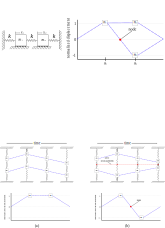
\includegraphics[width=\linewidth]{../figures/2-DOF_mode_shape.png}
	\caption{Modes of vibration for the system shown in figure \ref{fig:2-DOF-spring_mass_vertical} showing the: (a) first mode; and (b) second mode.}
	\label{fig:2-DOF_mode_shape}
\end{figure}
\end{example}

\subsection{Eigenvalue-based Solution for Natural Frequencies and Mode Shapes}

The process of calculating the mode shapes presented in section \ref{sec:two_degree_of_freedom} is long and tedious. Therefore, methods that can be easily deployed on computers are of great interest to the practitioner. An eigenvalue-based solution that takes advantage of the symmetry in the $M$ and $K$ matrices and can be easily implemented on a computer is discussed in this section. 

\begin{review}

	\textbf{Eigenvalues and Eigenvectors}

	In linear algebra, eigenvalues ($\lambda$) and eigenvectors ($\vec{v}$) are concepts that appear prominently in the analysis of linear transformations. By definition, If  $\vec{v}$ is a vector (in vector space $V$ over a field $F$) and $T$ is a linear transformation into itself, then $\vec{v}$ is an eigenvector of $T$ if $T(\vec{v})$ is a scalar multiple of $\vec{v}$:
	\begin{equation}
	T(\vec{v}) = \lambda\vec{v}
	\end{equation}
	where $\lambda$ is a scalar in the field $F$, known as the eigenvalue associated with the eigenvector $\vec{v}$. If the linear transformation is expressed in the form of an $n \times n$ matrix $\textbf{A}$, then the eigenvalue equation for a linear transformation above can be rewritten as the matrix multiplication
	\begin{equation}
	\textbf{A}\textbf{v} = \lambda\textbf{v}
	\end{equation}
	where $\textbf{v}$ is a $n \times 1$ matrix of the eigenvectors. For the matrix $A$, eigenvalues and eigenvectors can be used to decompose the matrix.

	\begin{figure}[H]
		\centering
		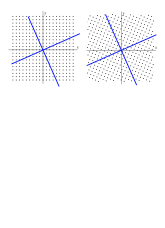
\includegraphics[]{../figures/eigenvalues.png}
		\caption{The stretching and shearing of the plane on which a matrix lies where the eigenvectors of the matrix are denoted by the blue lines and are the special directions such that point on the lines will just slide on them.}
		\label{fig:eigenvalues}
	\end{figure}

	The generalized eigenvalue problem is an important formulation for the study of vibrations and is written as 
	\begin{equation}
		\textbf{A}\textbf{v} = \vec{\lambda}\textbf{B}\textbf{v}
	\end{equation}	
	where $\textbf{A}$ and $\textbf{B}$ are real matrices. As written, this expression maps a general space $\textbf{A}$ into $\textbf{B}$ using $\vec{\lambda}$ and $\textbf{v}$. In the study of vibrations, the general generalized eigenvalue problem is used to link mass ($M$) and stiffness ($k$) matrices such that 
	\begin{equation}
		\textbf{K}\textbf{v} = \vec{\lambda}\textbf{M}\textbf{v}
	\end{equation}		
	
	
	

	\rd{Need to add a discussion on normal, orthogonal, and orthonormal matrices.}	






\end{review}

\begin{review}

\textbf{Cholesky Decomposition} 


	
	The Cholesky decomposition of a real positive-definite matrix $A$ is a decomposition of the form:
	\begin{equation}
		\textbf{A}=\textbf{LL}^{\text{T}}
		\end{equation}
	where $\textbf{L}$ is the lower triangular matrix of $\textbf{A}$. 	A matrix is positive definite if the scalar $\textbf{x}^{\text{T}}A\textbf{x}$ is positive for any non-zero vector $x$ comprised of real numbers:
	\begin{equation}
		\textbf{x}^{\text{T}}\textbf{A}\textbf{x} > 0
	\end{equation}


The vast majority of mass ($\textbf{M}$) and stiffness ($\textbf{K}$) matrices are symmetric and positive definite due to the physical meaning of these matrices. Therefore, $\textbf{M}$ can be factored into two terms using the Cholesky decomposition:
\begin{equation}
	M=LL^{\text{T}}
\end{equation}
For diagonal mass matrices (all the mass values lie along the diagonal of the matrix) the Cholesky decomposition ($L$) is defined as:
\begin{equation}
	L = M^{1/2} = \begin{bmatrix} \sqrt{m_1} & 0 \\  0  & \sqrt{m_2} \end{bmatrix} 
\end{equation}
This expression factors into:
\begin{equation}
	M = M^{1/2}M^{1/2}
\end{equation}
Moreover, the inverse of the diagonal matrix ($M^{1/2}$) is denoted as $M^{-1/2}$ and defined as:
\begin{equation}
	L^{-1} = M^{-1/2} = \begin{bmatrix} \frac{1}{\sqrt{m_1}} & 0 \\  0  & \frac{1}{\sqrt{m_2}} \end{bmatrix} 
\end{equation}
\end{review}


\subsubsection{Deriving the Eigenvalue-based Solution}
 
To derive an eigenvalue-based solution for calculating the natural frequencies and mode shapes let us consider the previously derived EOM for an undamped 2-DOF system:
\begin{equation}
M\ddot{\vec{x}} + K\vec{x} =0
\end{equation}
This expression can be transformed into a symmetric eigenvalue problem, allowing us to leverage the strengths of symmetric eigenvalue mathematics and computer solvers. To perform this transform, we set $\vec{x}=M^{-1/2}\vec{q}$ and multiply the equation by $M^{-1/2}$ such that the EOM becomes:
\begin{equation}
M^{-1/2}MM^{-1/2}\ddot{\vec{q}} + M^{-1/2}KM^{-1/2}\vec{q} =0
\end{equation}
As $M^{-1/2}MM^{-1/2}$ is equal to the identity matrix $I$ and defining $M^{-1/2}KM^{-1/2}$ as the mass normalized stiffness $\widetilde{K}$ yields the simplified expression:
\begin{equation}
I\ddot{\vec{q}} + \widetilde{K}\vec{q} =0
\end{equation}
where $\widetilde{K}=M^{-1/2}KM^{-1/2}$ is analogous to $\sqrt{k/m}$ from the 1-DOF system. 

As before, a solution is found by assuming a solution, taking the derivatives of the solution, and substituting it into the EOM. Following these steps and assuming a solution of:
\begin{equation}
\vec{q} = \textbf{v}e^{j\omega t}
\end{equation}
results in an EOM in the from:
\begin{equation}
-\textbf{v} \omega^2 e^{j\omega t} + \widetilde{K}\textbf{v}e^{j\omega t} =0
\end{equation}
driving out the nonzero scaler $e^{j\omega t}$ and rearranging the above expression results in:
\begin{equation}
\widetilde{K}\textbf{v} =  \omega^2 \textbf{v}
\end{equation}
Knowing that $\textbf{v}\neq0$, as a vector with zeros would mean no motion is present in the system, this equation can be expressed in a typical eigenvalue formulation:
\begin{equation}
\widetilde{K}\textbf{v} =  \lambda \textbf{v}
\label{eq:eigenvalue_problem}
\end{equation}
where $\lambda = \omega^2 $. Or more importantly, $\omega = \sqrt{\lambda}$. As $\widetilde{K}$ is symmetric, this is a symmetric eigenvalue problem. Moreover, the vector $\lambda$ represents the eigenvalues of the system. Given that we set $\vec{x}=M^{-1/2}\vec{q}$, the eigenvectors are not a direct representation of the mode shapes. To develop a link between the eigenvectors and mode shapes we first need to normalize the lengths of the eigenvectors obtained by solving equation \ref{eq:eigenvalue_problem} to that of a unit vector. The norm of a unit vector is defined as:
\begin{equation}
1= ||\textbf{v}|| = \sqrt{\textbf{v}^{\text{T}}\textbf{v}} = \sqrt{\sum_{i=1}^{n}(v_i^2)}
\end{equation} 
where a scalar is used in conjunction with vector such that $\alpha\textbf{u}=1$ computed the normalized unit vector directions as outlined in example \ref{ex:vector_normalizeation}. In general, a nonzero vector of any length can be normalized by calculating:
\begin{equation}
\frac{1}{\sqrt{\textbf{v}^{\text{T}}\textbf{v}} } \textbf{v}
\end{equation} 


We can relate the eigenvectors to the modes shapes by a factor of the mass matrix:
\begin{equation}
\vec{u}_1 = M^{-1/2}\vec{v}_1
\label{eq:modeshape_to_eigenvector}
\end{equation}
The important thing to remember is that the natural frequencies are the square root of the eigenvalues and the mode shapes are related to the eigenvectors through the mass matrix. 


\begin{example}
\label{ex:vector_normalizeation}
Normalize the vector $\vec{v}_1=[1/3 \hspace{1ex} 1]^\text{T}$

\textbf{Solution:} To normalize the vector $\vec{v}_1$, a scalar ($\alpha$) is calculated to make $\alpha\textbf{v}=1$.  Therefore, following the definition of an orthogonal vector:
\begin{equation}
(\alpha \vec{v}_1)^\text{T}(\alpha \vec{v}_1) = 1
\end{equation}
or:
\begin{equation}
\alpha [1/3 \hspace{1ex} 1]\alpha  \begin{bmatrix} \frac{1}{3}\\  1 \end{bmatrix}  = \alpha^2(1/9+1) = 1
\end{equation}
Therefore, $\alpha=3/\sqrt{10}$. Resulting in a normalized unit vector of $\alpha\vec{v}_1=[1/\sqrt{10} \hspace{1ex} 3/\sqrt{10}]^\text{T}$

\end{example}



\begin{example}
Consider the system presented in example \ref{ex:2-DOF} and repeated below where $m_1$=9 kg, $m_2$=1 kg, $k_1$ = 24 N/m, and $k_2$ = 3 N/m with the initial conditions $x_{10}=1$ mm, $v_{10}=0$ mm/s, $x_{20}=0$ mm, and $v_{20}=0$ mm/s. Calculate the natural frequencies and the mode shapes using the eigenvalue solution. 
\begin{figure}[H]
	\centering
	\includegraphics[]{../figures/2-DOF-spring_mass_horizontal.png}
	\caption{2-DOF system with two masses and two independent confidante systems $x_1$ and $x_2$.}
\end{figure}




\textbf{Solution:} Writing the mass and stiffness matrix of the system as:

\begin{equation}
	M = \begin{bmatrix} 9 & 0 \\  0  & 1 \end{bmatrix} 
\end{equation}
and 
\begin{equation}
	 K = \begin{bmatrix} 27 & -3 \\    -3  & 3 \end{bmatrix}
\end{equation}
we can compute  $\widetilde{K}$ using the following expression:
\begin{equation}
	 \widetilde{K}=M^{-1/2}KM^{-1/2}
\end{equation}
where $KM^{-1/2}$ is computed first to maintain symmetry. This results in:
\begin{equation}
	 KM^{-1/2} =  \begin{bmatrix} 27 & -3 \\    -3  & 3 \end{bmatrix}  \begin{bmatrix} \frac{1}{3} & 0 \\    0  & 1 \end{bmatrix}= \begin{bmatrix} 9 & -3 \\    -1  & 3 \end{bmatrix}
\end{equation}
and:
\begin{equation}
	  \widetilde{K}=M^{-1/2}KM^{-1/2} =  \begin{bmatrix} \frac{1}{3} & 0 \\    0  & 1 \end{bmatrix} \begin{bmatrix} 9 & -3 \\    -1  & 3 \end{bmatrix} =  \begin{bmatrix} 3 & -1\\  -1  & 3 \end{bmatrix} 
\end{equation}
Now a solution must be obtained for the eigenvalue problem:
\begin{equation}
\widetilde{K}\textbf{v} =  \lambda \textbf{v}
\end{equation}
While this can be obtained using computers for such a simple case it is more appropriate to solve this expression by had. Therefore, the above expression can be rewritten as:
\begin{equation}
(\widetilde{K} - \lambda I)\textbf{v} =  0
\end{equation}
as $\textbf{v} \neq 0$ the matrix must be singular, resulting in the determinant of the matrix equaling zero. Or:
\begin{equation}
\det \begin{bmatrix} 3-\lambda & -1 \\    -1  & 3-\lambda \end{bmatrix}  =  0
\end{equation}
This can be expanded ot the characteristic equation:
\begin{equation}
\lambda^2 -6\lambda + 8  =  0
\end{equation}
with the roots (eigenvalues):
\begin{equation}
\lambda_1 = 2\text{ and } \lambda_2 = 4
\end{equation}
Therefore, $\omega_1=\sqrt{2}$ and $\omega_2=2$. These are the same values computed in example \ref{ex:2-DOF}. The eigenvectors for $\lambda_1$ are computed as:
\begin{equation}
(\widetilde{K} - \lambda_1 I)\textbf{v} =  0
\end{equation}
or:
\begin{equation}
\begin{bmatrix} 3-2 & -1 \\    -1  & 3-2 \end{bmatrix} \begin{bmatrix} v_{11} \\ v_{21}  \end{bmatrix} =  \begin{bmatrix} 0 \\ 0  \end{bmatrix}
\end{equation}
This results in two dependent scalar equations:
\begin{equation}
v_{11} - v_{21} = 0 \text{ and } -v_{11} + v_{21} =0
\end{equation}
That show us that $v_{11} = v_{21}$ or $\vec{v}_1=[1 \hspace{1ex} 1]^\text{T}$. Therefore, using $(\alpha \vec{v}_1)^\text{T}(\alpha \vec{v}_1) = 1$ we obtain:
\begin{equation}
\alpha [1 \hspace{1ex} 1]\alpha  \begin{bmatrix} 1 \\  1 \end{bmatrix}  = \alpha^2(2) = 1
\end{equation}
or $\alpha = 1/\sqrt{2}$. This allows us to normalize the vector knowing $\alpha \vec{v}_1=1$, resulting in a normalized vector of:
\begin{equation}
\alpha \vec{v}_1=  \frac{1}{\sqrt{2}} \begin{bmatrix} 1 \\ 1 \end{bmatrix} 
\end{equation} 
A similar processes is followed for $\lambda_2=4$ that leads to the normalized vector 
\begin{equation}
\alpha \vec{v}_2=  \frac{1}{\sqrt{2}} \begin{bmatrix} -1 \\ 1 \end{bmatrix} 
\end{equation} 
Lastly, the normalized eigenvectors can be converted to mode shapes using $\textbf{u} = M^{-1/2}\textbf{v}$. Resulting in: 
\begin{eqnarray}
\vec{u}_1 =  \begin{bmatrix} \frac{1}{3} & 0  \\  0 & 1 \end{bmatrix}   \begin{bmatrix} 1 \\  1 \end{bmatrix} =  \begin{bmatrix} \frac{1}{3} \\  1 \end{bmatrix}
\end{eqnarray}
and:
\begin{eqnarray}
\vec{u}_2 =  \begin{bmatrix} \frac{1}{3} & 0  \\  0 & 1 \end{bmatrix}   \begin{bmatrix} -1 \\  1 \end{bmatrix} =  \begin{bmatrix} -\frac{1}{3} \\  1 \end{bmatrix}
\end{eqnarray}
Therefore, the first mode shape is $[1 \hspace{1ex} 1]$ while the second mode shape is $[\frac{1}{3} \hspace{1ex} -\frac{1}{3}]$. Again, this is using our prior definition of mode shapes to set $[1 \hspace{1ex} 1]$ as the first mode shape. Note that these are the same mode shape vectors as computed in example \ref{ex:2-DOF}.
\end{example}

Expanding on equation \ref{eq:modeshape_to_eigenvector}, the one can go from the eigenvector to the mode shapes through:
\begin{equation}
\vec{u}_1 = M^{-1/2}\vec{v}_1 \; \text{ and } \; \vec{v}_1 = M^{1/2}\vec{u}_1
\end{equation}
therefore, it can be seen that the eigenvectors and mode shapes are related through the term $\vec{v}_1$. 





%\section{forced vibration analysis}
%5.6 in Gao has a section of mechanical impedance



\subsection{Transfer-function method}

As in 1-DOF systems, transfer functions can be used to solve for the temporal response of 2-DOF systems under a variety of inputs. Again, the transfer function of a differential equation is defined as the ratio of the Laplace transform of the output (system response) to the Laplace transform of the input (forcing function). Moreover, the procedure for using the Laplace transform to solve the equations of motion is the same and follows three steps:
\begin{enumerate}
	\item Take the Laplace transform of both sides of the EOM while treating the time derivatives symbolically.
	\item Solve for $X(s)$ in the obtained equation.
	\item Apply the inverse transform $x(t) = \Laplace{X(s)}^{-1}$
\end{enumerate}


\begin{example}
\textbf{2-DOF System Subjected to Impulse}

Two masses are connected thorough a spring, as shown in figure~\ref{fig:2-DOF-spring_mass_free}. 
\begin{figure}[H]
	\centering
	\includegraphics[]{../figures/2-DOF-spring_mass_free.png}
	\caption{2-DOF system subjected to an impulse showing: (a) system, and (b) FBD. \rd{look at directions of arrow heads in (b), should some  point in?}}
	\label{fig:2-DOF-spring_mass_free}
\end{figure}
Assuming that $x_1$ displaces more than $x_2$, the equations of motion are:
\begin{eqnarray}
m_1\ddot{x}_1 + k(x_1-x_2)  = F_0 \delta (t) \\
m_2\ddot{x}_2 + k(x_2-x_1)  = 0  \nonumber
\end{eqnarray}
Taking the Laplace of both equations (step 1) yields:
\begin{eqnarray}
(m_1 s^2 +k)X_1(s) - k X_2(s) = F_0 \\
-k X_1(s) + (m_2 s^2 + k) X_2(s) = 0  \nonumber
\end{eqnarray}
solving these two equations for $X_1$ and $X_2$ (step 2) results in:
\begin{eqnarray}
X_1(s) = \frac{F_0(m_2 s^2 +k)}{s^2 [m_1 m_2 s^2 + k (m_1 + m_2)]} \\
X_2(s) = \frac{F_0 k}{s^2 [m_1 m_2 s^2 + k (m_1 + m_2)]} \nonumber
\end{eqnarray}
Using partial fractions, or a symbolic toolbox in MATLAB or Python, these expressions can be rewritten as:
\begin{eqnarray}
X_1(s) = \frac{F_0}{m_1 + m_2} \bigg( \frac{1}{s^2} + \frac{m_2}{\omega m_1} \frac{\omega}{s^2 + \omega^2} \bigg) \\
X_2(s) = \frac{F_0}{m_1 + m_2} \bigg( \frac{1}{s^2} + \frac{1}{\omega} \frac{\omega}{s^2 + \omega^2} \bigg) \nonumber
\end{eqnarray}
where:
\begin{equation}
\omega^2 = k \bigg( \frac{1}{m_1} + \frac{1}{m_2} \bigg)
\end{equation}
Taking the inverse transform of the expressions for $X_1(s)$ and $X_2(s)$ (step 3) results in expressions in the time domain and yields:
\begin{eqnarray}
x_1(t) = \frac{F_0}{m_1 + m_2} \bigg( t + \frac{m_2}{\omega m_1} \sin (\omega t) \bigg) \\
x_2(t) = \frac{F_0}{m_1 + m_2} \bigg( t + \frac{1}{\omega} \sin (\omega t) \bigg) \nonumber
\end{eqnarray}
Considering a system where $F_0=10$ N, $m_1=1000$ kg, $m_2=1000$ kg, and $k=1500$ N/m the temporal response is annotated in figure~\ref{fig:2_DOF_impact_example}. 


\begin{figure}[H]
	\centering
	\includegraphics[width=\linewidth]{../figures/2_DOF_impact_example.png}
	\caption{Temporal response for the considered 2-DOF system subjected to a impact load.}
	\label{fig:2_DOF_impact_example}
\end{figure}


\end{example}


\subsection{Cramer's Rule for Solving 2-DOF Systems}


\begin{figure}[H]
	\centering
	\includegraphics[]{../figures/2-DOF-spring_mass_dashpot_horizontal_double_wall.png}
	\caption{Forced 2-DOF damped system showing: (a) system, and (b) FBD. \rd{look at directions of arrow heads in (b), should some  point in?}}
	\label{fig:2-DOF-spring_mass_dashpot_horizontal_double_wall}
\end{figure}



Cramer's rule is an explicit formula for the solution of a system of linear equations with as many equations as unknowns. Cramer's rule is valid whenever the system has a unique solution and can be used as a more generalized approach to solving for the temporal solution to a 2-DOF. Consider the 2-DOF systems shown in figure~\ref{fig:2-DOF-spring_mass_dashpot_horizontal_double_wall}, where the two coupled equations of motion are expressed as: 
\begin{eqnarray}
m_1\ddot{x}_1 + (c_1+c_2)\dot{x}_1 - c_2\dot{x}_2 + (k_1+k_2)x_1 - k_2x_2 =0 \\
m_2\ddot{x}_2 + (c_2+c_3)\dot{x}_2 - c_2\dot{x}_1 + (k_2+k_3)x_2 - k_2x_1 =0 \nonumber
\end{eqnarray}
As before, taking the Laplace of the EOM (while ignoring the initial conditions) changes the equation from the temporal domain to the complex $s$-plane. This yields:
\begin{eqnarray}
m_1 s^2 X_1(s) + (c_1 + c_2)sX_1(s) - c_2sX_2(s) + (k_1+k_2)X_1(s) - k_2X_2(s) = F_1(s) \\
m_2 s^2 X_2(s) + (c_2 + c_3)sX_2(s) - c_2sX_1(s) + (k_2+k_3)X_2(s) - k_2X_1(s) = F_2(s) \nonumber
\end{eqnarray}
these equations can be rearranged in terms of $X_1$ and $X_2$ as follows:
\begin{equation}
[m_1 s^2 + (c_1 + c_2)s + (k_1+k_2)]X_1(s) - [c_2s+k_2]X_2(s) = F_1(s) 
\end{equation}
\begin{equation}
[m_2 s^2 + (c_2 + c_3)s + (k_2+k_3)]X_2(s) - [c_2s+k_2]X_1(s) = F_2(s) \nonumber
\end{equation}
These equations show two linear equations in terms of $X_1$ and $X_2$ that can be solved for using Cramer's rule, resulting in the expression:
\begin{eqnarray}
X_1(s) = \frac{D_1(s)}{D(s)} \\
X_2(s) = \frac{D_2(s)}{D(s)} \nonumber
\end{eqnarray}
where:
\begin{eqnarray}
D_1 = \left|
\begin{array}{cc}
F_1(s)  & -(c_2s+k_2) \\
F_2(s)  & m_2 s^2 + (c_2 + c_3)s + (k_2+k_3) \\
\end{array}
\right| \\
= [m_2 s^2 X_2(s) + (c_2 + c_3)s +(k_2+k_3)]F_1(s) + (c_2s+k_2)F_2(s)  \nonumber
\end{eqnarray}

\begin{eqnarray}
D_2 = \left|
\begin{array}{cc}
m_1 s^2 + (c_1 + c_2)s + (k_1+k_2)  & F_1(s) \\
-(c_2s+k_2)  & F_2(s) \\
\end{array}
\right| \\
= [m_1 s^2 + (c_1 + c_2)s + (k_1+k_2)]F_2(s) + (c_2s+k_2)F_1(s)  \nonumber
\end{eqnarray}

\begin{eqnarray}
D = \left|
\begin{array}{cc}
m_1 s^2 + (c_1 + c_2)s + (k_1+k_2) & m_2 s^2 + (c_2 + c_3)s + (k_2+k_3) \\
-(c_2s+k_2) & -(c_2s+k_2) \\
\end{array}
\right| \\ \nonumber
= m_1m_2s^4 + [m_2(c_1+c_3)+m_1(c_2+c_3)]s^3 \\  \nonumber
+ [m_2(k_1+k_2)+m_1(k_2+k_3)+c_1c_2+c_2c_3+c_3c_1]s^2 \\  \nonumber
+ [(k_1+k_2)(c_2+c_3)+c_1k_2+c_1k_3-c_2k_2+c_2k_3]s \\  \nonumber
+ (k_1k_2 + k_2k_3 + k_3k_1) \\  \nonumber
\end{eqnarray}

The denominator, $D(s)$ is a 4$^{\text{th}}$ polynomial in $s$ and is the characteristic polynomial of the system. The system is considered a 4$^{\text{th}}$ order system because the characteristic polynomial of the system is of order 4. 

\begin{example}
content...
content...
content...

\rd{Add an example}
% \rd{example 5.11 in Rao ed 6 has a good example of this nature.}
\end{example}

\subsection{Frequency Response Transfer Functions}

%\rd{Rao ed 5.11, p 526}


\subsection{Computational Methods for 2-DOF Systems}


% This works, but not sure how to get it to work with the major compile. 

\subsubsection{MATLAB}

\begin{example}
\textbf{Eigenvalue Problem}

\begin{figure}[H]
	\centering
	\includegraphics[]{../figures/2-DOF-spring_mass_horizontal.png}
	\caption{2-DOF system with two masses and two independent confidante systems $x_1$ and $x_2$.}
	\label{fig:2-DOF-spring_mass_horizontal_2}
\end{figure}

Using the Eigenvalue approach and MATLAB, determine the natural frequencies and mode shapes of the system shown in figure~\ref{fig:2-DOF-spring_mass_horizontal_2}, where $m_1$=9 kg, $m_2$=1 kg, $k_1$ = 24 N/m, and $k_2$ = 3 N/m with the initial conditions $x_{10}=1$ mm, $v_{10}=0$ mm/s, $x_{20}=0$ mm, and $v_{20}=0$ mm/s with the EOM expressed as: 
\begin{eqnarray}
  \begin{bmatrix} m_1 & 0  \\  0 & m_2 \end{bmatrix}\begin{bmatrix} \ddot{x_1} \\  \ddot{x_2} \end{bmatrix} + \begin{bmatrix} k_1+k_2 & -k_2  \\  -k_2 & k_2 \end{bmatrix}\begin{bmatrix} x_1 \\  x_2 \end{bmatrix} = \begin{bmatrix} 0 \\  0 \end{bmatrix}
\end{eqnarray}
Using the eigenvalue method, the following MATLAB code will solve for the natural frequencies and mode shapes:

%\lstinputlisting[caption = {Sample code from Matlab}]{code/matlab_eigenvalue_problem.m}
\lstset{linewidth=5.8in}
\begin{minipage}{1\textwidth}
	\begin{center}
		\lstset{%
			caption={MATLAB code to find the frequencies and mode shapes of a 2-DOF system.},
			basicstyle=\ttfamily\footnotesize\bfseries,
			frame=tb,
		}
		\begin{lstlisting}
% define the M and K matirx
M = [9 0; 0 1]
K = [24+3 -3; -3 3]

% build the M inverse squareroot and mass normalized stiffness matrix 
M_inv_sqr = sqrt(inv(M))
K_mass_norm = M_inv_sqr*K*M_inv_sqr

% Using, K_mass_norm*v=lambda*v
[v,lambda] = eig(K_mass_norm)

% Solve for natural frequencies
omega_1 = sqrt(lambda(1,1))
omega_2 = sqrt(lambda(2,2))

% solve for the mode shapes
u_1 = M_inv_sqr*v(:,1)
u_2 = M_inv_sqr*v(:,2)
		\end{lstlisting}
	\end{center}
\end{minipage}
\noindent where $\omega_1$=1.41 rad/sec and  $\omega_2$=2 rad/sec while $\vec{u}_1 = [0.333 \; 1]$ and $\vec{u}_2 = [-0.333 \; 1]$.

\end{example}


\begin{example}
\textbf{Roots of Quadratic Equation} \\
%\lstinputlisting[caption = {Sample code from Matlab}]{code/matlab_roots_of_quartic_equation.m}
\lstset{linewidth=5.8in}
\begin{minipage}{1\textwidth}
	\begin{center}
		\lstset{%
			caption={MATLAB code for time series responses of 1\textsuperscript{st} order system.},
			basicstyle=\ttfamily\footnotesize\bfseries,
			frame=tb,
		}
		\begin{lstlisting}
% for the function f(x) = x^4 -8x +12 =0
roots([1 0 0 -8 12]) 
		\end{lstlisting}
	\end{center}
\end{minipage}
\end{example}


\begin{example}
\textbf{Directly solving the ODE of the EOM for a 2-DOF system.} \\


	%\lstinputlisting[caption = {Function for Matlab code}]{code/matlab_function_dfunc.m}
	\lstset{linewidth=5.8in}
	\begin{minipage}{1\textwidth}
		\begin{center}
			\lstset{%
				caption={Function for Matlab code.},
				basicstyle=\ttfamily\footnotesize\bfseries,
				frame=tb,
			}
			\begin{lstlisting}
function f = matlab_function_dfunc(t,y)
	%UNTITLED Summary of this function goes here
	%   Detailed explanation goes here
	f=zeros(4,1)
	f(1) = y(2)
	f(2) = cos(3*t) - 4*y(2) + y(4) - 5*y(1) + 2*y(3)
	f(3) = y(2)
	f(4) = cos(3*t) + 0.5*y(2) - y(4) + y(1) - 1.5*y(3)
end 
			\end{lstlisting}
		\end{center}
	\end{minipage}





	%\lstinputlisting[caption = {Sample code from Matlab}]{code/matlab_temporal_response.m}
	\lstset{linewidth=5.8in}
	\begin{minipage}{1\textwidth}
		\begin{center}
			\lstset{%
				caption={Sample code from Matlab.},
				basicstyle=\ttfamily\footnotesize\bfseries,
				frame=tb,
			}
			\begin{lstlisting}
% define the time stamps of the system
tspan = [0: 0.1 : 20]

% define the initial conditions
y0 = [0.2; 1.0; 0.0; 8.0];

% solge the 2-DOF system using a ODE solver
[t,y] = ode23('matlab_function_dfunc',tspan, y0)

% plot the results
figure()
subplot(211)
plot(t,y(:,1))
xlabel('time (s)')
ylabel('x1(t) (m)')
subplot(212)
plot(t,y(:,3))
xlabel('time (s)')
ylabel('x1(t) (m)')
			\end{lstlisting}
		\end{center}
	\end{minipage}

\end{example}



\subsubsection{Python}




\subsection{Multiple Degrees of Freedom}

This chapter introduces methodologies for the solving of systems with more than 2-DOF. As shown in Chapter 5, 2-DOF systems can be solved analytically using 2 EOM coupled through their mode shapes. However, these methods become tedious when extended to systems with damping or even beyond the 2-DOF system.



\begin{example}
\textbf{Multiple Mode Shapes}



\begin{figure}[H]
	\centering
	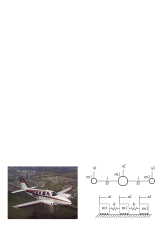
\includegraphics[width=\linewidth]{../figures/mode_shape_aiplane_example.png}
	\caption{A Beechcraft Baron in flight\protect\footnotemark[1] along with the Free-Free 3-DOF model simplified as a mass-spring model.}
	\label{fig:mode_shape_aiplane_example}
\end{figure}
\footnotetext[1]{``A Beechcraft Baron 58 in flight'' by San Diego Air \& Space Museum Archives, Public Domain.}  

Modeling the vibrations of a twin-engine airplane as a three-degree-of-freedom system can be done as shown in figure~\ref{fig:mode_shape_aiplane_example} where the fuselage is a center mass, and the engines are point masses suspended by cantilevers from the center mass. The stiffness of the wing corresponds to the modulus of the wing $E$ and its moment of inertia $I$. 
Assuming that $m_1=m_3=1m$, $m_2=3m$, and $k=\frac{3EI}{l}$, the EOM can be written as:

\begin{equation}
	  m\begin{bmatrix} 1 & 0 & 0 \\    0  & 3 & 0 \\ 0  & 0 & 1 \end{bmatrix} \begin{bmatrix} \ddot{x}_1 \\    \ddot{x}_2 \\    \ddot{x}_3  \end{bmatrix} + \frac{3EI}{l} \begin{bmatrix} 3 & -3 & 0 \\  -3  & 6 & -3 \\  0  & -3 & 3 \end{bmatrix} \begin{bmatrix} x_1 \\    x_2 \\    x_3 \end{bmatrix} = \begin{bmatrix} 0 \\  0 \\ 0 \end{bmatrix} 
\end{equation}
calculate the natural frequencies and mode shapes of the system and plot the mode-shapes in relation to the considered Beechcraft Baron.

\vspace{2ex}
\noindent \textbf{Solution using the mass normalized stiffness matrix $\tilde{K}$.}
\vspace{1ex}

Solving for the modes shapes using the  mass normalized stiffness matrix $\tilde{K}$ requires solving for $M^{-1/2}$ and $\tilde{K}$ such that:
\begin{equation}
	  M^{-1/2} = \begin{bmatrix} 1 & 0 & 0 \\    0  & 0.577 & 0 \\ 0  & 0 & 1 \end{bmatrix}
\end{equation}
\begin{equation}
	   \tilde{K} = M^{-1/2} K M^{-1/2} = \frac{3EI}{l} \begin{bmatrix} 3 & -1.732 & 0 \\  -1.732  & 2 & -1.732 \\  0  & -1.732 & 3 \end{bmatrix} 
\end{equation}
Than, the eigenvalue problem, formulated as:
\begin{equation}
\tilde{K} \textbf{v} = \lambda \textbf{v}
\end{equation}
is solved for the eigenvalues and eigenvectors, resulting in:
\begin{equation}
\lambda_1 = 0, \; \; \lambda_2 = 1.73, \; \; \lambda_3 = 2.23
\end{equation}
\begin{equation}
\vec{v}_1 = \begin{bmatrix} 0.44721 \\    0.77460 \\    0.44721  \end{bmatrix}, \; \; \vec{v}_2 = \begin{bmatrix} -0.707107 \\    0.0 \\    -0.707107 \end{bmatrix}, \; \; \vec{v}_3 = \begin{bmatrix} 0.54772 \\    -0.63245 \\    0.54772  \end{bmatrix}
\end{equation}
When the eigenvalue problem is solved using the mass normalized stiffness matrix $\tilde{K}$ the natural frequencies are $\omega_i = \sqrt{\lambda_i}$ while the mode shapes are derived from the eigenvectors as $\vec{u}=M^{-1/2}\vec{v}$. This results in:
\begin{equation}
\omega_1 = 0  \text{ rad/sec}, \; \; \omega_2 = 1.41421 \text{ rad/sec}, \; \; \omega_3 = 1.82574  \text{ rad/sec}
\end{equation}
\begin{equation}
\vec{u}_1 = \begin{bmatrix} 0.44721 \\   0.44721 \\    0.44721 \end{bmatrix}, \; \; \vec{u}_2 = \begin{bmatrix} -0.707107 \\    0.0 \\    -0.707107 \end{bmatrix}, \; \; \vec{u}_3 = \begin{bmatrix} 0.54772 \\    -0.36515 \\    0.54772  \end{bmatrix}
\end{equation}
Next, normalizing the mode shapes by the max of the vector which results in:
\begin{equation}
\vec{u}_1 = \begin{bmatrix} 1 \\    1 \\    1  \end{bmatrix}, \; \; \vec{u}_2 = \begin{bmatrix} -1 \\    0 \\    1 \end{bmatrix}, \; \; \vec{u}_3 = \begin{bmatrix} 1 \\    -0.667 \\    1  \end{bmatrix}
\end{equation}
these mode-shapes can than be plotted as:
\begin{figure}[H]
	\centering
	\includegraphics[width=\linewidth]{../figures/mode_shape_aiplane_example_normalized_stiffness.png}
	\caption{The unit vector normalized displacement of the mode shapes solved for using the mass normalized stiffness matrix $\tilde{K}$.}
	\label{fig:mode_shape_aiplane_example_normalized_stiffness}
\end{figure}



\vspace{2ex}
\noindent \textbf{Solution using the generalized eigenvalue approach.}
\vspace{1ex}

The mode shapes can also be solved for using the generalized eigenvalue approach where the eigenvalue problem is written as:
\begin{equation}
\textbf{K}\textbf{v} = \vec{\lambda}\textbf{M}\textbf{v}
\end{equation}
solving for the eigenvalues and eigenvectors yields:
\begin{equation}
\lambda_1 = 0, \; \; \lambda_2 = 1.73, \; \; \lambda_3 = 2.23
\end{equation}
\begin{equation}
v_1 = \begin{bmatrix} -0.57735 \\    -0.57735 \\   -0.57735  \end{bmatrix}, \; \; v_2 = \begin{bmatrix} 0.707107 \\    0.0 \\    -0.707107 \end{bmatrix}, \; \; v_3 = \begin{bmatrix} 0.63960 \\    -0.42640 \\    0.63960  \end{bmatrix}
\end{equation}
Note that the eigenvalues are the same as those solved for using the normalized stiffness matrix approach while the eigenvectors appear to be different. This is because for absolute value of the eigenvectors do not hold information as only their direction as a set matters. To get the same values, you must normalizing the mode shapes by the norm of the vector such that $\vec{u}_i = \frac{\vec{u}_i}{|\vec{u}_i|}$. While for the the generalized eigenvalue approach $u_i=v_i \alpha$ where $\alpha$ is a scaling value. Note that here $\alpha=1$ as the mode shapes are already normalized. Plotting the normalized mode shapes results in:

\begin{figure}[H]
	\centering
	\includegraphics[width=\linewidth]{../figures/mode_shape_aiplane_example_generalized_eigenvalue.png}
	\caption{The unit vector normalized displacement of the mode shapes solved for using the generalized eigenvalue approach.}
	\label{fig:mode_shape_aiplane_example_generalized_eigenvalue}
\end{figure}

Software tools and computing languages do not all follow the same standards in terms of returning normalized eigenvectors.  However, as the information stored in the eigenvectors is just the direction of the transform. Therefore, the mode shapes are correct but some amplitudes are reversed as the mode shapes only report the shape these are corrected.  For example, see mode shape 2 above, in each case the mode shape is the same, however, how it is presented is a matter of preference.




%Next, normalizing the mode shapes by the norm of the vector as $\vec{u}_i = \frac{\vec{u}_i}{|\vec{u}_i|}$ results in:
%\begin{equation}
%	\vec{u}_1 = \begin{bmatrix} 0.57735 \\    0.57735 \\    0.57735  \end{bmatrix}, \; \; \vec{u}_2 = \begin{bmatrix} -0.707107 \\    0.0 \\    0.707107 \end{bmatrix}, \; \; \vec{u}_3 = \begin{bmatrix} 0.666667 \\    -0.333333 \\    0.666667  \end{bmatrix}
%\end{equation}
%these mode-shapes can than be plotted as:



\end{example}




\subsection{Modal Analysis}

Modal analysis is the study of a system's dynamic properties and is done in the frequency domain. Consider a system with $n$ degrees of motion, modal analysis allows for the uncoupling of the EOM into $n$ single-degree-of-freedom system (represented as 2$^{\text{nd}}$-order DOF systems) where the displacements of the masses are expressed as the linear summations of the normal modes of the system. If every mode shape is considered, the solution is equivalent to the solution obtained from the original $n^{\text{th}}$-degree-of-freedom system. 

Consider the generic multidegree-of-freedom system under external forces, expressed as:


\begin{equation}
M \ddot{\vec{x}} + K\vec{x} = \vec{F}
\end{equation}


\noindent where damping is not considered and the vector $\vec{F}$ is a set of deterministic inputs. To expand this equation by modal analysis, the eigenvalue problem must first be solved. The generalized eigenvalue problem is written at: 

\begin{equation}
\lambda M \textbf{v} = K \textbf{v}
\end{equation}

For the $n^{\text{th}}$-degree-of-freedom, the generalized eigenvalue problem can be simplified to: 
\begin{equation}
\omega_i^2 M \vec{v}_i = K  \vec{v}_i
\end{equation}
Considering that the total displacement of the system, expressed as $\vec{x}(t)$ , is the summation of the of the displacement of each of the noncontributing modes; assuming a linear system, the temporal response of the system can be written as:
\begin{eqnarray}
\vec{x}(t) = q_1(t) \vec{v}_1 + q_2(t) \vec{v}_2 + q_3(t) \vec{v}_3 + \cdots + q_n(t) \vec{v}_n
\label{eq:combination_of_modes}
\end{eqnarray}
\noindent where the time-dependent generalized scalars $q_1(t), q_1(t), \cdots, q_1(t)$ are the modal participation coefficients (also called principal coordinates). Defining the modal matrix $P$ as: \todo{The v here is not eigenvector, it is $M^{-1/2}u_1$. }
\begin{equation}
P = [ \vec{v}_1 \; \; \vec{v}_2 \; \; \vec{v}_3 \cdots \vec{v}_n]
\end{equation}
Therefore, the linear combination of the normal modes (equation~\ref{eq:combination_of_modes}) can be more concisely written as:
\begin{equation}
\vec{x}(t) = P\vec{q}(t)
\end{equation}
where $\vec{q}(t) = [q_1 \; \; q_2 \; \; q_3 \cdots q_n]^{\text{T}}$. Next, the relationship that relates the physical space to the modal space for the acceleration component is written as:
\begin{equation}
\ddot{\vec{x}}(t) = P\ddot{\vec{q}}(t)
\end{equation}
combining these two terms results in the EOM that can be written as:
\begin{equation}
M P\ddot{\vec{q}}(t) + KP\vec{q}(t) = \vec{F}
\end{equation}
To convert the EOM into the standard form, first the $P^{\text{T}}$ is multiplied through the equation as:
\begin{equation}
P^{\text{T}} M P\ddot{\vec{q}}(t) + P^{\text{T}} K P\vec{q}(t) = P^{\text{T}} \vec{F}
\end{equation}
If the modes are normalized, the following is true: \todo{Should this be $\widetilde{K}$?}
\begin{equation}
P^{\text{T}} M P = I
\label{eq:modes_normalized}
\end{equation}
where $I$ is the identity matrix and 
\begin{equation}
P^{\text{T}} K P = \begin{bmatrix} \nwarrow & 0 & 0 \\  0  & \omega^2 & 0 \\  0  & 0 & \searrow \end{bmatrix}
\end{equation}



Moreover, defining $\vec{Q}(t) = P^{\text{T}} \vec{F}$ results in a EOM expressed as:
\begin{equation}
\ddot{\vec{q}}(t) +  \begin{bmatrix} \nwarrow & 0 & 0 \\  0  & \omega^2 & 0 \\  0  & 0 & \searrow \end{bmatrix} \vec{q}(t) = \vec{Q}(t)
\end{equation}
For a system with $n$ degrees of freedom, this equation can be broken down into:
\begin{equation}
\ddot{\vec{q}}_i(t) + \omega_i^2 \vec{q}_i (t) =  \vec{Q}(t), \; \; i=1,2, \cdots, n
\end{equation}
This expression is the same ODE that we have solved multiple times in this text. Therefore, we know the solution to be:
\begin{equation}
q_i(t) = q_{i0} \cos(\omega_i t) +  \frac{\dot{q}_{i0}}{\omega_i} \sin( \omega_i t)
\end{equation}
Lastly, to solve for a solution in the modal space, the initial conditions that were given in the physical space must be converted to the modal space. This can be done by generalizing the velocities in terms of the modal matrix:
\begin{equation}
\vec{q}(0) = P^\text{T} M \vec{x}(0)
\end{equation}
\begin{equation}
\dot{\vec{q}}(0) = P^\text{T} M \vec{v}(0)
\end{equation}


%\todo{test}

\begin{example}
\textbf{Free vibration response}

Solve for the free vibration response of the 2-DOF presented in figure~\ref{fig:2-DOF-spring_mass_horizontal_double_wall} using modal analysis. Show the temporal response for the entire system for its first 20 seconds using the full modal reconstruction and the reconstruction truncated to just include the first mode. Also, plot the variations in the modal participation coefficients though time. Apply the parameters, $f_1 = 0$ kg, $f_2 = 0$ N, $m_1 = 10$ kg, $m_2 = 1$ kg, $k_1 = 30$ N/m, $k_2 = 5$ N/m, $k_3 = 1$ N/m, $x_1(0) = 1$ mm, $x_2(0) = 0$ mm, $v_1(0) = 0$ mm, and $v_2(0) = 0$ mm.

\begin{figure}[H]
	\centering
	\includegraphics[]{../figures/2-DOF-spring_mass_horizontal_double_wall.png}
	\caption{Forced 2-DOF damped system showing: (a) system, and (b) FBD.}
	\label{fig:2-DOF-spring_mass_horizontal_double_wall}
\end{figure}


The equations of motion that couple the system are:
\begin{eqnarray}
m_1\ddot{x}_1 + (k_1+k_2)x_1 - k_2x_2 = 0 \\
m_2\ddot{x}_2 + (k_2+k_3)x_2 - k_2x_1 = 0 \nonumber
\end{eqnarray}
In matrix form, these become:

\begin{equation}
	  \begin{bmatrix} m_1 & 0 \\    0  & m_2 \end{bmatrix} \begin{bmatrix} \ddot{x}_1 \\    \ddot{x}_2  \end{bmatrix} + \begin{bmatrix} k_1 + k_2 & -k_2 \\  -k_2  & k_2 + k_3 \end{bmatrix} \begin{bmatrix} x_1 \\    x_2  \end{bmatrix} = \begin{bmatrix} 0 \\  0  \end{bmatrix} 
\end{equation}
\begin{equation}
	  \vec{x}(0) = \begin{bmatrix} 1 \\  0 \end{bmatrix},\; \; \vec{v}(0) = \begin{bmatrix} 0 \\  0 \end{bmatrix} \nonumber
\end{equation}
The natural frequencies and mode shapes can than be obtained by solving the eigenvalue problem. Setting up the generalized eigenvalue problem: \rd{look at symmetric M and K matrices} %\rd{these are symmetric M and K matrices so I don't know why $\tilde{K}$ does not work in a normal eigenvalue problem. Maybe norms of vectors? It is not simple scaling. This example is based off or Rao 6.16 6ed} \rd{I think it has to do with solving the generalized eigenvalue matrix vs the mass normalized one and when you apply the second M$^{-1/2}$ as you need it all the time. }
\begin{equation}
K \textbf{v} = \lambda M \textbf{v}
\end{equation}
and solving yields:
\begin{equation}
\lambda_1 = 2.734 \text{, } \vec{v}_1 = \begin{bmatrix} 0.546819 \\  0.837251 \end{bmatrix} 
\end{equation}
\begin{equation}
\lambda_2 = 6.765 \text{, } \vec{v}_2 = \begin{bmatrix} -0.151349 \\  0.988480 \end{bmatrix}  \nonumber
\end{equation}
this is then related to the natural frequency and mode shapes as:
\begin{equation}
\omega_1 = \sqrt{\lambda_1} = 1.65 \text{ rad/s, } \vec{v}_1 = \vec{v}_1 \alpha_1 = \begin{bmatrix} 0.546819 \\  0.837251 \end{bmatrix} \alpha_1
\end{equation}
\begin{equation}
\omega_2 = \sqrt{\lambda_2} = 2.60 \text{ rad/s, } \vec{v}_2 = \vec{v}_2 \alpha_2 = \begin{bmatrix} -0.151349 \\  0.988480 \end{bmatrix} \alpha_2 
\end{equation}
recall that the eigenvalues only contain information about the direction of the linear transform, and therefore, there magnitudes are arbitrary.Therefore, they must be scaled proportionally to each other. For this reason, the scalars $\alpha_1$ and $\alpha_2$ are added. My orthogonalizing the modal vectors with respect to the mass matrix, the values of $\alpha_1$ and $\alpha_2$ are found as:
\begin{equation}
1 = \vec{v}_1^\text{T} M \vec{v}_1 
\end{equation}
\begin{equation}
1 = \alpha_1^2 \begin{bmatrix} 0.546819 &  0.837251 \end{bmatrix} \begin{bmatrix} 10 & 0 \\    0  & 1 \end{bmatrix}  \begin{bmatrix} 0.546819 \\  0.837251 \end{bmatrix}
\end{equation}
and:
\begin{equation}
1 = \vec{v}_2^\text{T} M \vec{v}_2 
\end{equation}
\begin{equation}
1 = \alpha_2^2 \begin{bmatrix} -0.151349 &  0.98848 \end{bmatrix} \begin{bmatrix} 10 & 0 \\    0  & 1 \end{bmatrix}  \begin{bmatrix} -0.151349 \\  0.98848 \end{bmatrix}
\end{equation}
therefore, $\alpha_1=0.520$ and $\alpha_2=0.910$. Now, applying the proper scaling values to the modal vector, the modal matrix becomes:
\begin{equation}
P = [ \vec{v}_1 \; \; \vec{v}_2 ] = \begin{bmatrix} 0.284 & -0.137 \\    0.435  & 0.900 \end{bmatrix}
\end{equation}
Next, check that the normal modes in the modal matrix ($P$) are normalized, per equation~\ref{eq:modes_normalized}. This yields,
\begin{equation}
P^{\text{T}} M P = \begin{bmatrix} 1 & -2.775e-16 \\   -2.775e-16 & 1 \end{bmatrix} \approx I
\end{equation}
which is close enough to I. Considering that $\vec{x}(t) = P\vec{q}(t)$, the EOM for the system can be expressed as:
\begin{equation}
\ddot{\vec{q}}(t) + \begin{bmatrix} \omega_1^2 & 0 \\    0  & \omega_2^2 \end{bmatrix} \vec{q} (t) = \vec{Q} = \begin{bmatrix} 0 \\  0  \end{bmatrix} 
\end{equation}
rewriting this in scalar form for each modal coefficient yields:
\begin{equation}
\ddot{q}_i(t) + \omega_i^2 q_i (t) = 0, \; \; i=1,2
\end{equation}
where the solution for this ODE is:
\begin{equation}
q_i(t) = q_{i0} \cos(\omega_i t) +  \frac{\dot{q}_{i0}}{\omega_i} \sin( \omega_i t)
\end{equation}
where $q_{i0}$ and $\dot{q}_{i0}$ are the initial conditions in modal space. Therefore, the given initial conditions must be transferred into modal space as:
\begin{equation}
\vec{q}(0) = P^\text{T} M \vec{x}(0) = \begin{bmatrix} 0.284 &  0.435 \\  -0.137    & 0.900 \end{bmatrix} \begin{bmatrix} 10 & 0 \\  0  & 1 \end{bmatrix}  \begin{bmatrix} 1 \\  0 \end{bmatrix} =  \begin{bmatrix}  2.846 \\  -1.378 \end{bmatrix}
\end{equation}
\begin{equation}
\dot{\vec{q}}(0) = P^\text{T} M \vec{v}(0) = \begin{bmatrix} 0.284 &  0.435 \\  -0.137    & 0.900 \end{bmatrix} \begin{bmatrix} 10 & 0 \\  0  & 1 \end{bmatrix}  \begin{bmatrix} 0 \\  0 \end{bmatrix} =  \begin{bmatrix}  0 \\  0 \end{bmatrix}
\end{equation}
therefore, 
\begin{eqnarray}
q_1(t) = 2.846 \cdot \cos (1.65 t) \\ 
q_2(t) = -1.378 \cdot \cos (2.6 t)  \nonumber
\label{eq:participation}
\end{eqnarray}
converting back into the time domain is done knowing $\vec{x}(t) = P\vec{q}(t)$, therefore, 
\begin{equation}
\vec{x}(t) = P\vec{q}(t) = \begin{bmatrix} 0.284 & -0.137 \\    0.435  & 0.900 \end{bmatrix}  \begin{bmatrix} 2.846 \cdot \cos (1.65 t) \\  -1.378 \cdot \cos (2.6 t) \end{bmatrix}
\end{equation}
This further simplified into:
\begin{eqnarray}
x_1(t) = 0.808 \cdot \cos (1.65 t) + 0.189 \cdot \cos (2.6 t) \\ 
x_2(t) = 1.238 \cdot \cos (1.65 t) - 1.240 \cdot \cos (2.6 t)  \nonumber
\end{eqnarray}
These results are plotted in figure~\ref{fig:modal_analysis_free_vibration}.
\begin{figure}[H]
	\centering
	\includegraphics[width=\linewidth]{../figures/modal_analysis_free_vibration.png}
	\caption{Temporal response for the 2-DOF reconstructed using just all the modal coordinates.}
	\label{fig:modal_analysis_free_vibration}
\end{figure}

Next, the truncated response can be computed by only considering the first mode response for the system (i.e. $\vec{x}(t) = q_1(t) \vec{v}_1$). This is obtain as:

\begin{equation}
\vec{x}(t) = P\vec{q}_\text{truncated}(t) = \begin{bmatrix} 0.284 & -0.137 \\    0.435  & 0.900 \end{bmatrix}  \begin{bmatrix} 2.846 \cdot \cos (1.65 t) \end{bmatrix}
\end{equation}
This further simplified into:
\begin{eqnarray}
x_1(t) = 0.808 \cdot \cos (1.65 t) \\ 
x_2(t) = 1.238 \cdot \cos (1.65 t) \nonumber
\end{eqnarray}
These results are plotted in figure~\ref{fig:modal_analysis_free_vibration_truncated}. Note that this only considers the response of the system that is a function of the first mode. Note that this captures some of the ``general'' idea of the system while missing out on the finer points that the 2$^{\text{nd}}$ mode contributes. 

\begin{figure}[H]
	\centering
	\includegraphics[width=\linewidth]{../figures/modal_analysis_free_vibration_truncated.png}
	\caption{Truncated temporal response for the 2-DOF reconstructed using just the first modal coordinates.}
	\label{fig:modal_analysis_free_vibration_truncated}
\end{figure}

Lastly, the participation of the two modes can be plotted from the time series response of equation~\ref{eq:participation}.

\begin{figure}[H]
	\centering
	\includegraphics[width=\linewidth]{../figures/modal_analysis_free_participation_factors.png}
	\caption{Modal participation coefficients.}
	\label{fig:modal_analysis_free_participation_factors}
\end{figure}



\end{example}



\end{document}
















% Chapter 6 Vibration Control
\documentclass[12pt,letter]{article}
\usepackage{mathptmx} % added for time new roman font
\usepackage[left=1in,right=1in,top=1in,bottom=1in]{geometry}
\usepackage[latin1]{inputenc}
\usepackage{amsmath}

% defines all example enviorment
\usepackage[framemethod=tikz]{mdframed} % added for the box around examples
\newtheorem{ex}{Example}
\numberwithin{ex}{section} % allows for the use of example numbers that lign up with the section numbers
\newenvironment{example}{\begin{mdframed}[middlelinewidth=0.5mm]\begin{ex}\normalfont}{\end{ex}\end{mdframed}}

% defines all review enviorment
\usepackage[framemethod=tikz]{mdframed} % added for the box around examples
\newtheorem{re}{Review}
\numberwithin{re}{section} % allows for the use of example numbers that lign up with the section numbers
\newenvironment{review}{\begin{mdframed}[middlelinewidth=2mm,roundcorner=20pt]\begin{re}\normalfont}{\end{re}\end{mdframed}}

% defines all vibration case studies
\newtheorem{vcs}{Vibration Case Studies}
\numberwithin{vcs}{section} % allows for the use of numbers that lign up with the section numbers
\newenvironment{vibration_case_studies}{\begin{mdframed}[linecolor=orange,middlelinewidth=2mm,roundcorner=20pt]\begin{vcs}\normalfont}{\end{vcs}\end{mdframed}}

% defines the quotation enviorment 
\usepackage{xcolor}
\newcommand{\quotebox}[2]{\begin{center}\fcolorbox{white}{blue!15!gray!15}{\begin{minipage}{0.9\linewidth}\vspace{10pt}\center\begin{minipage}{0.8\linewidth}{\space\Huge``}{#1}{\Huge''}{\break\null\hfill} {\small #2}  \end{minipage}\medbreak\end{minipage}}\end{center}}

% defines the definition enviorment 
\newcommand{\definitionbox}[2]{\begin{center}\fcolorbox{white}{blue!15!gray!15}{\begin{minipage}{0.9\linewidth}\vspace{10pt}\center\begin{minipage}{0.8\linewidth} {{\textbf{Definition} - }{#1}: {#2}}\end{minipage}\medbreak\end{minipage}}\end{center}}

\usepackage{amsfonts}
\usepackage{amssymb}
\usepackage{graphicx}
\usepackage{float}
\usepackage{booktabs}
%\usepackage{parskip} % remove all the paragraph indents
\usepackage[textsize=tiny]{todonotes}
\usepackage[OT2, T1]{fontenc}			% added for Russian names in Cryillic text
\usepackage[russian, english]{babel}	% added for Russian names in Cryillic text
\usepackage{enumitem}					% added to reduce the space in itemized list

\usepackage{setspace}
\usepackage[colorlinks=true]{hyperref}
\usepackage{textcomp} 
\usepackage{multicol} 

% added for MATLAB code
\usepackage[framed]{matlab-prettifier}
\let\ph\mlplaceholder % shorter macro
\lstMakeShortInline"

\lstset{
	style              = Matlab-editor,
	basicstyle         = \mlttfamily,
	escapechar         = ",
	mlshowsectionrules = true,
}



\usepackage{color} % color added for editing
\newcommand{\bl}[1]{\textcolor[rgb]{0.00,0.00,1.00}{#1}}
\newcommand{\gr}[1]{\textcolor[rgb]{0.00,0.50,0.00}{#1}}
\newcommand{\rd}[1]{\textcolor[rgb]{0.75,0.00,0.00}{#1}}
\newcommand{\tl}[1]{\textcolor[rgb]{0,0.6,0.60}{#1}}



%%%%%%%		define the symbols for positive directions		%%%%%%
\makeatletter													%%	
%%					
\newcommand*\curveplus{% positive counterclockwise				%%
	\mathbin{\rotatebox[origin=c]{90}{$\m@th\curvearrowleft$}+}}	%%
%%
\newcommand*\rightplus{% positive right							%%
	\mathpalette\@rightplus\relax}								%%
\newcommand*\@rightplus[1]{%									%%
	\mathbin{\vcenter{\hbox{$\m@th\overset{#1+}{\to}$}}}}			%%
%%	
\newcommand*\upplus{% positive up								%%
	\mathbin{+\mathord\uparrow}}									%%
%%			
\newcommand*\downplus{% positive down							%%		
	\mathbin{+\mathord\downarrow}}								%%
%%		
\newcommand*\downrightplus{% positive down and right			%%	
	\mathbin{+ \rotatebox[origin=c]{-30}{$\m@th\rightarrow$}}}	%%
\makeatother 													%%	
%%%%%%%%%%%%%%%%%%%%%%%%%%%%%%%%%%%%%%%%%%%%%%%%%%%%%%%%%%%%%%%%%%


\usepackage{mathtools}          %loads amsmath as well added for the piece wise function
\DeclarePairedDelimiter\Floor\lfloor\rfloor
\DeclarePairedDelimiter\Ceil\lceil\rceil


\newcounter{NumberInTable}
\newcommand{\LTNUM}{\stepcounter{NumberInTable}{(\theNumberInTable)}}

\newcommand{\Laplace}[1]{\ensuremath{\mathcal{L}{\left[#1\right]}}}
\newcommand{\InvLap}[1]{\ensuremath{\mathcal{L}^{-1}{\left[#1\right]}}}
\renewcommand{\textuparrow}{$\uparrow$}

% Sets the footnotes to be letters, not numbers. This is needed or it's a mix of both. 
\renewcommand*\thefootnote{\alph{footnote}}


\begin{document}
	
	% set the section number, along with figure and equation numbers
	\setcounter{section}{5}	
	\setcounter{figure}{0}   
	\renewcommand\thefigure{\thesection.\arabic{figure}}
	\setcounter{equation}{0}   
	\renewcommand\theequation{\thesection.\arabic{equation}}

	\section{Vibration Control}

Throughout this text, we have studied various aspects related to analyzing and modeling vibrating systems. Therefore, it becomes prudent to look at methods for reducing or eliminating unwanted vibrations. However, before vibrations in a system can be effectively reduced they must be better understood in terms of their effects on the system under study. For this reason, this chapter first introduces the vibration Nomograph, this is then followed by vibration isolation, absorption, and active suppression.  

\subsection{Vibration Nomograph}

\begin{figure}[tp!]
    \centering
    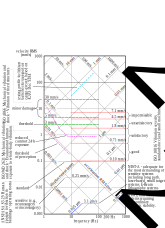
\includegraphics[width=6.5in]{../figures/Vibration_nomograph}
    \caption{Vibration nomograph showing the acceptable limits of vibration for various applications.}
    \label{fig:Vibration_nomograph}
\end{figure}


There exist various methods and standards for measuring and describing acceptable levels of vibrations in systems, these include ISO/AWI 2631 for the evaluation of human exposure to whole-body vibrations and ISO 4866 for the measurement and effects of vibrations on structures. A common way to present the acceptable limit of vibration is in a vibration nomograph.  A vibration nomograph is a simplified way to express the acceptable limits on a system while considering the displacement, velocity, acceleration, and frequency of a system. A typical nomograph with various limits is presented in figure \ref{fig:Vibration_nomograph}. 

A vibration nomograph is a logarithmic plot that allows us to easily express the relationships between displacement, velocity, acceleration, and frequency of a system. The vibration nomograph presented in figure \ref{fig:Vibration_nomograph} considers an undamped 1-DOF system with constant amplitude ($A$) experiencing harmonic motion that can be modeled as:
\begin{equation}
    x(t) = A \sin(\omega t)
    \label{eq:displacement}
\end{equation}
Therefore, the velocity and acceleration terms can be found by taking the derivatives of the displacement expression to yield:
\begin{equation}
    \dot{x}(t) = A \omega \cos(\omega t)
\end{equation}
and:
\begin{equation}
    \ddot{x}(t) = -A\omega^2 \sin(\omega t)
    \label{eq:acceleration}
\end{equation}
These equations are converted from a circular frequency in rad/sec to a linear frequency ($f$) in Hz, such that $\omega = 2\pi f$. Therefore, equations \ref{eq:displacement}-\ref{eq:acceleration} become:
\begin{equation}
    x(t) = A \sin(\omega t)
\end{equation}
\begin{equation}
    v(t) =  \dot{x}(t) = 2\pi f A \cos(\omega t)
\end{equation}
\begin{equation}
    a(t) =  \ddot{x}(t) = -4\pi^2 f^2 A \sin(\omega t)
\end{equation}
Thereafter, the maximum values for velocity $v_\text{max}$ and acceleration $a_\text{max}$ are related to amplitude through:
\begin{equation}
    v_\text{max} = 2\pi f A 
    \label{eq:v_max}
\end{equation}
\begin{equation}
    a_\text{max} = -4\pi^2 f^2 A = -2 \pi f v_\text{max}
    \label{eq:a_max}
\end{equation}
by taking the natural log of both side of equation \ref{eq:v_max} we obtain: 
\begin{equation}
    \ln v_\text{max} = \ln(2\pi f) + \ln A
    \label{eq:ln_v_max} 
\end{equation}
doing the same for equation \ref{eq:a_max} leads to:
\begin{equation}
     \ln a_\text{max} = - \ln(2\pi f) - \ln v_\text{max}
    \label{eq:ln_v_max_2} 
\end{equation}
It can be seen that both of these expressions are linear. 



The nomograph sets the $x-$axis as frequency in Hz and the $y-$axis as velocity in mm/s. Equation \ref{eq:ln_v_max} tells us that For a constant amplitude of displacement ($A$), $\ln v_\text{max}$ is linearly proportional to $\ln (2 \pi f)$, at a rate of $2 \pi$. As the $x-$axis in a nomograph is frequency, measured in Hz and thereby accounting for the $2 \pi$, $\ln (2 \pi f)$ is a straight line with a positive slope of 1 with respect the frequency axis (i.e. $x-$axis). Therefore, a line on the nomograph that represents a constant displacement is at a 45$^\circ$ angle from the $x$-axis. 


For a constant value of velocity, ($v_\text{max}$), equation \ref{eq:ln_v_max_2} shows that acceleration ($\ln a_\text{max}$) is linearly proportional to $-\ln (2 \pi f)$, at a rate of $2 \pi$. Again, as the $x-$axis in a nomograph is frequency, measured in Hz, acceleration is represented by a straight line that varies with $- \ln(2\pi f)$, therefore, $\ln a_\text{max}$ is a straight line with the slope of -1. This is also represented by a line of constant acceleration set at a -45$^\circ$ angle from the $x$-axis. These equations are expressed in the vibration nomograph plot of figure \ref{fig:Vibration_nomograph} where each point on the plot represents a specific sinusoidal (harmonic) vibration for a 1-DOF system.  



		\begin{vibration_case_studies}
	Discuss hot tire thread is off-set to control the pitch created by road noise.
	\begin{figure}[H]
		\centering
		\includegraphics[width=4.5in]{../figures/tire_tred_patent.png}
		\caption{Illustration for US patent US2006197A which proposed the use of irregular thread patterns to control the pitch of road noses\protect\footnotemark[1].}
	\end{figure}	
	\footnotetext[1]{Public Domain} 	
\end{vibration_case_studies}








\subsection{Vibration Isolation}

% Vibration isolation of electronics. 


To mitigate vibrations on a system the ideal approach would be to limit the source of vibrations. However, this is not always applicable to the system you are considering. Therefore, isolating the system from vibrations in the next best step. One approach to this is to design systems around limiting the force and displacement transmissibility discussed prior; where both force and displacement transmissibility  are considered \emph{isolation problems}.

One way to do this is to track the \emph{transmissibility ratio} which is denoted at T.R. and defines the ratio of the magnitude of the transmitted $(F_T)$ to applied force $(F_0)$. 

\begin{equation}
	\text{T.R.} = \frac{F_T}{F_0} = \sqrt{\frac{1+(2 \zeta \beta )^2}{(1-\beta^2)^2+(1 \zeta \beta )^2}}
\end{equation}

%%%%%%%%%%%%%%%%%%%%%%%%%%%%%%%%%%%%%%%%%%%%%%%%%%%%%%%%%%%%%%%%%%%%%%%%%%%%%%%%%%%%%%%%%%%%%%%%%
%  \todo{add exmaple on vibration isolation for electronics. Use example form shock test system.}
%%%%%%%%%%%%%%%%%%%%%%%%%%%%%%%%%%%%%%%%%%%%%%%%%%%%%%%%%%%%%%%%%%%%%%%%%%%%%%%%%%%%%%%%%%%%%%%%%


\subsection{Vibration Absorption}

Vibration absorbers, also termed dynamic vibration absorber, are a class of mechanical devices that seek to reduce unwanted vibrations in a system. In contrast to a traditional dash-pot style damper, these systems seek to ``redirect'' the vibrations from the system to another mass connected to the system. In this way the main system is protected form the bandwidth of vibrations that the vibration absorbers is tuned for. As the vibration absorbers must be tuned for the system, it is generally limited to devices that operate at a fixed frequency like industrial equipment or cables suspended in the air and subjected to wind loading. Figure~\ref{fig:vibration_absorbers} presents a Stockbridge and a Dogbone damper designed to remove certain bandwidths of excitation form wind-excited cables.

\begin{figure}[H]
    \centering
    \includegraphics[width=6.5in]{../figures/vibration_absorbers}
    \caption{Vibration absorbers deployed on wind excited cables showing: (a) a Stockbridge damper on a high-power transmission line\protect\footnotemark[1], and; (b) a dogbone damper on a suspender cable of a suspension bridge\protect\footnotemark[2].}
    \label{fig:vibration_absorbers}
\end{figure}
\footnotetext[1]{``Stockbridge dampers installed on high voltage power lines'' by Badics CC BY-SA 3.0}  
\footnotetext[2]{``Dogbone dampers on the road-support cables of the Severn Bridge'' by Bassaar  CC BY-SA 4.0}  

Vibration absorbers are most often designed to shift the resonance frequency of the first mode of the system away from the expected excitation frequency. This is done by adding an additional degree-of-freedom in the form of a mass (the vibration absorber) connected to system with a spring to alter the natural frequency of the combined system away from the original excitation frequency. Dashpots may also be added in parallel to the spring element if additional energy dissipation in needed beyond that provided by the original system. 

\begin{figure}[H]
    \centering
    \includegraphics[]{../figures/vibration_absorber_spring_mass.png}
    \caption{A vibration absorber ($m_2$) for mitigating unwanted dynamics in a device ($m_1$).}
    \label{fig:vibration_absorber_spring_mass}
\end{figure}

The tuning of a 2-DOF system can be done by setting the displacement of the mass to be controlled to zero and solving for the mass and stiffness of vibration absorber. Consider the system presented in figure~\ref{fig:vibration_absorber_spring_mass}, here $m_1$ and $k_1$ are the mass and stiffness of the system while $m_2$ and $k_2$ are the mass and stiffness of the vibration absorber. A good assumption to make when designing a vibration absorber is that the mass of the absorber should be between 1\% and 5\% of the mass of the system to be damped. Therefore, for this case let $m_1$ = 20 kg, $m_2$ = 1 kg, and $k_1$ = 20 kN. Assuming a sinusoidal input where $F_0 = 1$ kN, the equations of motion are:
\begin{equation}
m_1\ddot{x_1} + k_1 x_1 + k_2(x_1-x_2)  = F_0 \sin (\omega t)
\end{equation}
\begin{equation}
m_2\ddot{x_2} + k_2(x_2-x_1) = 0
\end{equation}
Assuming the temporal solution is of a harmonic form, the following is true:
\begin{equation}
x_i(t) = X_i \sin (\omega t ), \; \; i=1,2
\end{equation}
using the transfer function approach and assuming no initial conditions, the following steady state solution can be obtained for $m_1$ and $m_2$:
\begin{equation}
X_1 = \frac{(k_2 - m_2 \omega^2)F_0}{(k_1+k_2-m_1 \omega^2)(k_2-m_2 \omega^2) -k_2^2}
\label{eq:X1_displacement}
\end{equation}
\begin{equation}
X_2 = \frac{k_2 F_0}{(k_1+k_2-m_1 \omega^2)(k_2-m_2 \omega^2) -k_2^2}
\label{eq:X2_displacement}
\end{equation}
Next, the natural frequency of $m_1$ ($\omega_1$) can be solved for as $\omega_1=\sqrt{k_1 / m_1}$. In order to eliminate movement for $m_1$ at a given driving frequency $\omega$, the numerator of equation~\ref{eq:X1_displacement} should be set to zero. Note that setting $F_0$ is a trivial solution and provides no real benefit to the system. Therefore:
\begin{equation}
k_2 = m_2 \omega^2
\end{equation}
note that this will force the frequency of the tuned vibration absorber to match that of the system, therefore $\omega_1 = \omega_2 = \sqrt{k_2 / m_2}$. Next, normalizing the input force $F_0$ by the stiffness of the main system $k_1$ yields:
\begin{equation}
\delta_{\text{st}} = \frac{F_0}{k_1}
\end{equation}
using this term, equations~\ref{eq:X1_displacement} and \ref{eq:X2_displacement} can be rearranged as:
\begin{equation}
\frac{X_1}{\delta_{\text{st}}} = \frac{1 - \big(\frac{\omega}{\omega_2} \big)^2 }{\Big[1 + \frac{k_2}{k_1} - \big(\frac{\omega}{\omega_1} \big)^2 \Big] \Big[ 1- \big(\frac{\omega}{\omega_2} \big)^2 \Big] -\frac{k_2}{k_1}}
\label{eq:X1_norm_displacement}
\end{equation}
\begin{equation}
\frac{X_2}{\delta_{\text{st}}} = \frac{1}{\Big[1 + \frac{k_2}{k_1} - \big(\frac{\omega}{\omega_1} \big)^2 \Big] \Big[ 1- \big(\frac{\omega}{\omega_2} \big)^2 \Big] -\frac{k_2}{k_1}}
\label{eq:X2_norm_displacement}
\end{equation}
Figure~\ref{fig:vibration_absorber_undamped_results} reports the normalized displacement of the system over a frequency range for system with and without a vibration absorber. Note that at $\omega=1$ the original system is in resonance while the system with the vibration absorber has no displacement. However, no system is without compromise. From equation~\ref{eq:X2_norm_displacement} it can be seen that at $\omega = \omega_1 = \omega_2$ the second mass needs a displacement equal to:
\begin{equation}
X_2 = -\frac{k_1}{k_2}\delta_{\text{st}} = -\frac{F_0}{k_2}
\end{equation}
or 1 m using the given parameters. Therefore, the mass and stiffness values of the vibration absorber should be selected based the the allowable travel of the absorber (i.e. $X_2$), among other factors. Moreover, from this equation it can be seen the force exerted by the second mass operates in the direction opposite the original force ($-F_0 - k_2 X_2$), thereby canceling it. Lastly, note that the addition of the vibration absorber creates two resonate frequencies of the system, termed $\Omega_1$ and $\Omega_2$. These  resonate frequencies represent roots of the system and care should be taken to limit the time the system spends at these frequencies (i.e. on startup). The locations of these roots can be solved for analytically by setting the denominators of equation \ref{eq:X1_norm_displacement} to zero.

%%%%%%%%%%%%%%%%%%%%%%%%%%%%%%%%%%%%%%%%%%%%%%%%%%%%%%%%%%%%%%%%%%%%%%%%%%%%%%%%%%%%%%%%%%%%%%%%
%  \todo{Add text on the mass and frequency ratios $\mu$ and $\beta$.}
%%%%%%%%%%%%%%%%%%%%%%%%%%%%%%%%%%%%%%%%%%%%%%%%%%%%%%%%%%%%%%%%%%%%%%%%%%%%%%%%%%%%%%%%%%%%%%%%

\begin{figure}[H]
    \centering
    \includegraphics[width=6.5in]{../figures/vibration_absorber_undamped_results.png}
    \caption{Frequency response of the undamped system with and without the vibration absorber.}
    \label{fig:vibration_absorber_undamped_results}
\end{figure}



\begin{vibration_case_studies}
	Tuned mass dampers for vibration mitigation in tall structures
	\begin{figure}[H]
		\centering
		\includegraphics[width=3.5in]{../figures/Taipei_101_Tuned_Mass_Damper.png}
		\caption{Illustration of Taipei 101's main tuned mass damper. \protect\footnotemark[1]}
	\end{figure}
	
	A tuned mass dampers (TMD), also known as a harmonic absorber or seismic damper, are devices that are designed into a structure to mitigate structural vibration. The mass is typically a block of steel or concrete and is mounted on suspended cables to create a pendulum and damped in relation to the structure. By tuning the oscillating frequency of the damping system to be near the same natural frequency of the structure, energy is transferred to the mass and extracted through the dampers. Thereby reducing vibration which prevents discomfort or damage. While discussed here in the context of tall buildings, tuned mass dampers are also frequently found in automobile components and power transmission lines.	
	
\footnotetext[1]{Someformofhuman, CC BY-SA 4.0 $<$https://creativecommons.org/licenses/by-sa/4.0$>$, via Wikimedia Commons} 	
\end{vibration_case_studies}



\subsection{Active Vibration Suppression}

Vibrations in systems can be mitigated through a number a active systems; typically its easiest to consider this as an actuator that add energy to the system at the correct time to cancel out vibrations. 

\subsubsection{Metrics for vibration control}

There are various performance indicators that one can use to judge the performance of an active control scheme. They depend on the system order (1\textsuperscript{st}, 2\textsuperscript{nd}) and the excitation experienced by the system. For simplicity in this introductory text, we will define four performance indicators subjected to a step response, each shown in figure~\ref{fig:2nd_order_performance_indicators}. The performance indicators are:
\begin{itemize}[itemsep=0.25ex,topsep=0.25ex]
	%\item rise time $ \rightarrow t_\text{r}$
	\item peak time  ($t_\text{p}$) is the time to the first peak.
	\item peak value  ($x_\text{p}$) is the maximum value experiences by the system
	\item settling time ($t_\text{s}$) is the time it take the system to get within an error ($\pm \epsilon \%$) of the steady-state displacement ($x_{ss}$) and stay there.
	% \item delay time  $ \rightarrow t_\text{d}$
	\item max percentage overshoot ($M_\text{p}$) is defined as $M_p = ( {x_p} / {x_{ss}}-1 ) \cdot 100$.
\end{itemize}

\begin{figure}[H]
	\centering
	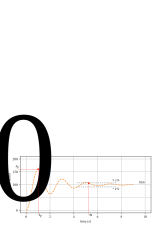
\includegraphics[]{../figures/2nd_order_performance_indicators}
	\label{fig:2nd_order_performance_indicators}
\end{figure}












\subsubsection{Position-Derivative (PD) Control}

Active vibration control add energy to the system in order to mitigate the vibrations in the system. As depicted in figure \ref{fig:active_vibration_control_FBD}(a), an active vibration control system requires a sensor to acquire data from the system, control hardware and algorithms to processes this data, and an actuator to exert a physical control on the system. These system together are called a feedback loop, as a movement in the mass results in a control force $(f_u)$ being exerted on the system. This control force is diagrammed in figure \ref{fig:active_vibration_control_FBD}(b). 

\begin{figure}[H]
    \centering
    \includegraphics[width=5in]{../figures/active_vibration_control_FBD.png}
    \caption{Active vibration control system showing: (a) the system with a feed-back loop that takes a signal from the sensor, converts it to a control signal, and drives the actuator; and (b) the free body diagram.}
    \label{fig:active_vibration_control_FBD}
\end{figure}


Adding the control force to the EOM for the 1-DOF system presented in figure \ref{fig:active_vibration_control_FBD} results in:
\begin{equation}
m \ddot{x} + c \dot{x} + kx = F(t) = f + f_u
\end{equation}
A common method for providing control for vibration suppression is called position and derivative control or PD-control. A PD-controller is a state-variable feedback controller as it uses velocity and displacement obtained from the measured acceleration, assuming that the acceleration is properly integrated. PD-control measures the position and velocity of the mass and uses these to compute the control force needed to mitigate the vibration to an acceptable level. A simple way to code a PD-controller is to provide a control force proportional to the displacement velocity (derivative of displacement) of the mass such that:
\begin{equation}
f_u = -g_1x - g_2 \dot{x}
\end{equation}
where $g_1$ and $g_2$ are the proportional gains of the systems. The control gains can be constants determined by the designer or variables updated through time by an algorithm. Here we will consider the gains to be constant, therefore, the EOM for the closed-loop system in figure \ref{fig:active_vibration_control_FBD} becomes:
\begin{equation}
m \ddot{x} + (c + g_2) \dot{x} + (k + g_1)x = F(t) = f 
\end{equation}
This formulation lets $g_1$ act as additional stiffness while $g_2$ acts as additional damping. This closed-loop EOM can be used to solve for the effective natural frequency of the system, given by:
\begin{equation}
\omega_n = \sqrt{\frac{k+g_1}{m}}
\end{equation}
and the effective damping ratio of the system
\begin{equation}
\zeta = \frac{c+g_2}{2\sqrt{m(k+g_1)}}
\end{equation}


\subsubsection{Proportional-Integral-Derivative (PID) Control}

Proportional-Integral-Derivative (PID) Control is a three-term controller that employs feedback that is widely used in continuous control systems, including for the control of structural systems. A PID controller seeks to minimize the measured error value $e(t)$ between a desired setpoint (SP) and a measured process variable (PV) by applying correctios based on the proportional ($P$), integral ($I$), and derivative ($D$) terms (denoted P, I, and D respectively), from which it gets its name.

\begin{figure}[H]
	\centering
	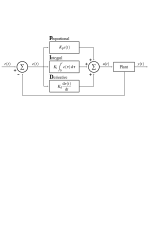
\includegraphics[]{../figures/PID_controller.png}
	\caption{Generalized PID controller for a system with feedback, where $r(t)$ is the desired setpoint (SP) and $y(t)$ is the measured process value (PV).}
	\label{fig:PID_controller}
\end{figure}

The overall control equation is defined as
\begin{equation}
	u(t) = K_\text{p} e(t) + K_\text{i} \int_0^t e(\tau) \,\mathrm{d}\tau + K_\text{d} \frac{\mathrm{d}e(t)}{\mathrm{d}t}
\end{equation}
where where $K_\text{p}$, $K_\text{i}$, and $K_\text{d}$ are non-negative coefficients for the proportional, integral, and derivative terms, respectively. The PID controller is diagrammed in figure~\ref{fig:PID_controller} for a system with feedback control, such as that shown in figure~\ref{fig:active_vibration_control_FBD}. Moreover, in the Laplace domain the transfer function of the PID controller is defined as
\begin{equation}
	\Laplace{s} = K_\text{p} + \frac{K_\text{i}}{s} + K_\text{d}s
\end{equation}
where $s$ is the complex frequency. A temporal response for the 1-DOF shown in figure~\ref{fig:active_vibration_control_FBD} when controlled with a PID controller is reported in figure~\ref{fig:PID_temporal_response_1}.

\begin{figure}[H]
	\centering
	\includegraphics[]{../figures/PID_temporal_response_1.png}
	\caption{System response for a 1-DOF system controlled with a PID.}
	\label{fig:PID_temporal_response_1}
\end{figure}



\begin{review}
	\label{sec:control_systems_review}
	
		Continuous control systems have been widely used for centuries. For example, consider that the centrifugal governor which uses spinning weights was used by Christiaan Huygens in the 1600s in the Netherlands to regulate the gap between millstones in windmills or by James Watt who famously linked a stem regulator to a centrifugal governor to control steam turbines. 

		Arguably, the Russian American engineer Nicolas Minorsky was the first to develop the theoretical analysis for the three-term control we now call PID. This was done in 1922 while he was researching and designing automatic ship steering for the US Navy. He based his work on watching how a ship's helmsman responds to wave loading on a ship, with a delayed input to the helm that not only considered the current ship course, but also past error and the desired rate of change for the ship. For a helmsman, the goal is stability, not absolute control, which simplifies how one thinks about the challenge of control.
		
	\begin{figure}[H]
		\centering
		\includegraphics[width=6in]{../figures/PID_Nicolas_Minorsky_and_USS_New_Mexico}
		\caption{Historical prospective of PID control showing: (a) Portrait of Nicolas Minorsky \protect\footnotemark[1] and (b) the battleship USS New Mexico (BB-40) of the United States Navy which was the first to implement PID control in its steering \protect\footnotemark[2]. }
		\label{fig:fragility_curve}
	\end{figure}

	\footnotetext[1]{Peter Minorsky, grandson of Nicolas Minorsky, CC BY-SA 1.0 $<$https://creativecommons.org/licenses/by-sa/1.0$>$, via Wikimedia Commons} 
	\footnotetext[2]{U.S. Navy, Public domain, via Wikimedia Commons} 
	
\end{review}






%
%\subsubsection{Linear-Quadratic Regulator (LQR) Control}
%








%	Use this code just to build the bibliography items and copy them out of the bbl file into the text above. This is the only way I was able to get the reference to show up when the entire text is compiled. 
	\pagebreak
	\renewcommand{\thepage}{}
	\renewcommand\refname{References Cited}
	\pagestyle{plain}
	\bibliographystyle{unsrtDOI}
	\bibliography{Chapter_6_vibration_control}






















			


	
\end{document}
















% Chapter 7 Structural Dynamics
\include{Chapter_7_structural_dynamics/Chapter_7_structural_dynamics}
%
%%% Chapter 8 Signal Processing
%\documentclass[12pt,letter]{article}
\usepackage{mathptmx} % added for time new roman font
\usepackage[left=1in,right=1in,top=1in,bottom=1in]{geometry}
\usepackage[latin1]{inputenc}
\usepackage{amsmath}

% defines all example enviorment
\usepackage[framemethod=tikz]{mdframed} % added for the box around examples
\newtheorem{ex}{Example}
\numberwithin{ex}{section} % allows for the use of example numbers that lign up with the section numbers
\newenvironment{example}{\begin{mdframed}[middlelinewidth=0.5mm]\begin{ex}\normalfont}{\end{ex}\end{mdframed}}

% defines all review enviorment
\usepackage[framemethod=tikz]{mdframed} % added for the box around examples
\newtheorem{re}{Review}
\numberwithin{re}{section} % allows for the use of example numbers that lign up with the section numbers
\newenvironment{review}{\begin{mdframed}[middlelinewidth=2mm,roundcorner=20pt]\begin{re}\normalfont}{\end{re}\end{mdframed}}

% defines all vibration case studies
\newtheorem{vcs}{Vibration Case Studies}
\numberwithin{vcs}{section} % allows for the use of numbers that lign up with the section numbers
\newenvironment{vibration_case_studies}{\begin{mdframed}[linecolor=orange,middlelinewidth=2mm,roundcorner=20pt]\begin{vcs}\normalfont}{\end{vcs}\end{mdframed}}

% defines the quotation enviorment 
\usepackage{xcolor}
\newcommand{\quotebox}[2]{\begin{center}\fcolorbox{white}{blue!15!gray!15}{\begin{minipage}{0.9\linewidth}\vspace{10pt}\center\begin{minipage}{0.8\linewidth}{\space\Huge``}{#1}{\Huge''}{\break\null\hfill} {\small #2}  \end{minipage}\medbreak\end{minipage}}\end{center}}

% defines the definition enviorment 
\newcommand{\definitionbox}[2]{\begin{center}\fcolorbox{white}{blue!15!gray!15}{\begin{minipage}{0.9\linewidth}\vspace{10pt}\center\begin{minipage}{0.8\linewidth} {{\textbf{Definition} - }{#1}: {#2}}\end{minipage}\medbreak\end{minipage}}\end{center}}

\usepackage{amsfonts}
\usepackage{amssymb}
\usepackage{graphicx}
\usepackage{float}
\usepackage{booktabs}
%\usepackage{parskip} % remove all the paragraph indents
\usepackage[textsize=tiny]{todonotes}


\usepackage{setspace}
\usepackage[colorlinks=true]{hyperref}
\usepackage{textcomp} 
\usepackage{multicol} 

% added for MATLAB code
\usepackage[framed]{matlab-prettifier}
\let\ph\mlplaceholder % shorter macro
\lstMakeShortInline"

\lstset{
	style              = Matlab-editor,
	basicstyle         = \mlttfamily,
	escapechar         = ",
	mlshowsectionrules = true,
}



\usepackage{color} % color added for editing
\newcommand{\bl}[1]{\textcolor[rgb]{0.00,0.00,1.00}{#1}}
\newcommand{\gr}[1]{\textcolor[rgb]{0.00,0.50,0.00}{#1}}
\newcommand{\rd}[1]{\textcolor[rgb]{0.75,0.00,0.00}{#1}}
\newcommand{\tl}[1]{\textcolor[rgb]{0,0.6,0.60}{#1}}



%%%%%%%		define the symbols for positive directions		%%%%%%
\makeatletter													%%	
%%					
\newcommand*\curveplus{% positive counterclockwise				%%
	\mathbin{\rotatebox[origin=c]{90}{$\m@th\curvearrowleft$}+}}	%%
%%
\newcommand*\rightplus{% positive right							%%
	\mathpalette\@rightplus\relax}								%%
\newcommand*\@rightplus[1]{%									%%
	\mathbin{\vcenter{\hbox{$\m@th\overset{#1+}{\to}$}}}}			%%
%%	
\newcommand*\upplus{% positive up								%%
	\mathbin{+\mathord\uparrow}}									%%
%%			
\newcommand*\downplus{% positive down							%%		
	\mathbin{+\mathord\downarrow}}								%%
%%		
\newcommand*\downrightplus{% positive down and right			%%	
	\mathbin{+ \rotatebox[origin=c]{-30}{$\m@th\rightarrow$}}}	%%
\makeatother 													%%	
%%%%%%%%%%%%%%%%%%%%%%%%%%%%%%%%%%%%%%%%%%%%%%%%%%%%%%%%%%%%%%%%%%


\usepackage{mathtools}          %loads amsmath as well added for the piece wise function
\DeclarePairedDelimiter\Floor\lfloor\rfloor
\DeclarePairedDelimiter\Ceil\lceil\rceil


\newcounter{NumberInTable}
\newcommand{\LTNUM}{\stepcounter{NumberInTable}{(\theNumberInTable)}}

\newcommand{\Laplace}[1]{\ensuremath{\mathcal{L}{\left[#1\right]}}}
\newcommand{\InvLap}[1]{\ensuremath{\mathcal{L}^{-1}{\left[#1\right]}}}
\renewcommand{\textuparrow}{$\uparrow$}

% Sets the footnotes to be letters, not numbers. This is needed or it's a mix of both. 
\renewcommand*\thefootnote{\alph{footnote}}


\begin{document}
	
	% set the section number, along with figure and equation numbers
	\setcounter{section}{7}	
	\setcounter{figure}{0}   
	\renewcommand\thefigure{\thesection.\arabic{figure}}
	\setcounter{equation}{0}   
	\renewcommand\theequation{\thesection.\arabic{equation}}

	\section{Experimental Vibrations}
	
Experimental vibration testing requires the practitioner to understand the basics of testing hardware and digital signal processing.


\begin{vibration_case_studies}

	On August 14, 2018, the Ponte Morandi viaduct in Genoa Italy collapsed, killing 43 and displacing hundreds of people from their homes. The Morandi viaduct was a cable-stayed bridge with uniquely few stays, typically only two per span. The Stays were a hybrid of steel cables overlaid with concrete. The concrete overlay made the direct inspection of the stays impossible. 
	
	While the exact cause may never be known, is suspected that one of the stay cables within the concrete failed due to corrosion and poor maintenance causing a bridge with very little redundancy in its design to fail\protect\footnotemark[1].
	
	In 2017, researchers from the Polytechnic University of Milan instrumented and studied the vibration characteristics of the bridge and noted that the modal frequencies of the stays on pillar 9 (the one that collapsed) were more than 10\% different than other stays on the bridge. While it's always hard to draw conclusions from one text, comparing modal frequencies between two similar structures can be useful for tracking damage. 
 
	\begin{figure}[H]
		\centering
		\includegraphics[width=6in]{../figures/ponte_morandi_bridge}
		\caption{The Ponte Morandi bridge, showing the bridge: a) before the collapse\protect\footnotemark[2], and; b) after collapse\protect\footnotemark[3]. }
	\end{figure}
		
	\footnotetext[1]{Rymsza, Janusz. ``Causes of the Collapse of the Polcevera Viaduct in Genoa, Italy.'' Applied Sciences 11, no. 17 (2021): 8098. https://doi.org/10.3390/app11178098.} 	
	\footnotetext[2]{Davide Papalini, CC BY-SA 3.0 $<$https://creativecommons.org/licenses/by-sa/3.0$>$, via Wikimedia Commons} 
	\footnotetext[3]{Michele Ferraris, CC BY-SA 4.0 $<$https://creativecommons.org/licenses/by-sa/4.0$>$, via Wikimedia Commons} 
\end{vibration_case_studies}
		
		
\subsection{Hardware for vibration testing}

The measurements of vibrations requires specialized hardware. While an variety of vendors sell vibration measurement systems in a number of form factors, the general hardware requirements remain constant. To study the dynamic response of systems subjected to a wide range of excitation, the basic hardware requirements are: \emph{Exciter} - A system to provide a measurable input to the system, \emph{Transducers} - Sensors used for converting the mechanical movements of the structure, and \emph{data acquisition} - Hardware for digitizing the the signal generated by the transducers.

\begin{figure}[H]
	\centering
	\includegraphics[]{../figures/vibration_testing.png}
	\caption{Key components for performing experimental modal analysis.}
	\label{fig:vibration_testing}
\end{figure} 




 

\begin{figure}[H]
    \centering
    \includegraphics[width=6.5in]{../figures/accelerometers}
    \caption{Integrated Electronics Piezo-Electric (IEPE) accelerometers, showing: (a) the cross section of a typical IEPE) accelerometer with key components annotated, and; (b) selection of IEPE accelerometers for various applications.}
    \label{fig:accelerometers}
\end{figure} 








\begin{table}[H]
\caption{Parameters for various IEPE accelerometers.}
\resizebox{\textwidth}{!}{\begin{tabular}{@{}llllll@{}}
\toprule
\multicolumn{1}{c}{parameter} & \multicolumn{5}{c}{accelerometers} \\ \midrule
model number & PCB 393B31 & PCB  393B04 & PCB 352C67 & PCB 352A21 & PCB 352A92 \\
Sensitivity($\pm$ 10 \%) & 10.0 V/g & 1000 mV/g & 100 mV/g & 10 mV/g & 0.25 mV/g \\
Measurement Range & $\pm$ 0.5 g pk & $\pm$ 5 g pk & $\pm$ 50 g pk & $\pm$ 500 g pk & $\pm$ 20 kg pk \\
Frequency Range($\pm$ 5 \%) & 0.1 to 200 Hz & 0.06 to 450 Hz & 0.5 to 10 kHz & 1.0 to 10 kHz & 1.2 to 10 kHz \\
Resonant Frequency & \textgreater 700 Hz & \textgreater 2.5 kHz & \textgreater 35 kHz & \textgreater 50 kHz & \textgreater 100 kHz \\
Non-Linearity & $\le$1\% & $\le$1\% & $\le$1\% & $\le$1\% &  \\
Transverse Sensitivity & $\le$5\% & $\le$5\% & $\le$5\% & $\le$5 \% &  \\ \bottomrule
\end{tabular}}
\end{table}


\begin{figure}[H]
	\centering
	\includegraphics[width=3.5in]{../figures/frequency_rolloff}
	\caption{frequency rolloff.\protect\footnotemark[1] }
	\label{fig:frequency_rolloff}
\end{figure}

\footnotetext[1]{PDerivative work:  KrishnavedalaOriginal:  Omegatron, CC BY-SA 3.0 $<$https://creativecommons.org/licenses/by-sa/3.0$>$, via Wikimedia Commons}






%Measurement Range & 0.5 g pk & \pm 5 g pk & \pm 50 g pk & \pm 100 g pk & \pm 500 g pk & \pm20,000 g pk \\
%Frequency Range(\pm 5 \%) & 0.1 to 200 Hz & 0.06 to 450 Hz & 0.5 to 10,000 Hz & 1 to 5,000 Hz & 1.0 to 10,000 Hz & 1.2 to 10,000 Hz \\


\begin{figure}[H]
    \centering
    \includegraphics[width=6.5in]{../figures/IEPE.png}
    \caption{Integrated Electronics Piezo-Electric (IEPE)-based measurement system showing the: (a) simplified circuit schematic\protect\footnotemark[1]; and (b) IEPE data acquisition systems in various form factors.}
    \label{fig:IEPE}
\end{figure} 


A modal hammer is used to impart a measured impact into the structure. Figure~\ref{fig:modal_hammer} shows a model hammer with interchangeable tips and the responses generated by the tips. 

\begin{figure}[H]
	\centering
	\includegraphics[width=6.5in]{../figures/modal_hammer.png}
	\caption{Model hammer with interchangeable tips.}
	\label{fig:modal_hammer}
\end{figure} 



\footnotetext[1]{``IEPE sensor connected to the input of an instrument'' by JanBurg  CC BY-SA 4.0}  



\pagebreak


\subsection{Digital Signal Processing}


	\begin{review}
	\label{sec:Laplace_review}
		
		Harry Nyquist (February 7, 1889 ? April 4, 1976) was a Swedish physicist and electronic engineer. His parents emigrated to the U.S. in 1907.  He attended the University of North Dakota starting in 1912 where he obtained a B.S. in 1914 and an M.S. in 1915, both in electrical engineering (entry to M.S. was 3 years!). Thereafter, he went to Yale University where he received a Ph.D. in physics in 1917.

		\begin{figure}[H]
			\centering
			\includegraphics[width=2.71in]{../figures/Harry_Nyquist.jpg}
			\caption{Picture of Harry Nyquist from the American Institute of Physics.\protect\footnotemark[1]}
			\label{fig:fragility_curve}
		\end{figure}
		\footnotetext[1]{Fair use, via Wikimedia Commons}
	\end{review}



\begin{figure}[H]
    \centering
    \includegraphics[width=6.5in]{../figures/signal_digitization.png}
    \caption{Digitization of two continuous time-series signals sampled at 5 S/s.}
    \label{fig:signal_digitization}
\end{figure}


The Nyquist-Shannon sampling theorem is a theorem in the field of signal processing that defines the sample rate that permits a discrete sequence of samples (i.e. discrete-time) to sample a continuous-time signal of finite bandwidth. 

\begin{figure}[H]
    \centering
    \includegraphics[width=6.5in]{../figures/aliasing.png}
    \caption{Aliasing of a 3 Hz signal that is sampled at 5 S/s.}
    \label{fig:aliasing}
\end{figure}

In signal processing, aliasing is an effect that causes different signals to become indistinguishable from each other.  In this way, the signals become an alias of one another when sampled. Aliasing also accounts for the development of distortion or artifact in a reconstructed signal when compared to the original continuous signal.


\begin{figure}[H]
    \centering
    \includegraphics[width=6.5in]{../figures/spectrogram.png}
    \caption{Spectrogram of a 0-10 Hz chirp signal.}
    \label{fig:spectrogram}
\end{figure}

Some of the key parameters in a spectrogram include:

\begin{itemize}
\item window
\item segment length
\item overlap
\end{itemize}


\subsection{Frequency response function}









\end{document}




















\pagebreak
\renewcommand{\thepage}{}
\renewcommand\refname{References Cited}
\pagestyle{plain}
\bibliographystyle{Downey_NSF}
\bibliography{Chapter_1_Basic_Concepts}


















\end{document}

